% LaTeX .tex example for the proceedings of
% COBEM 2011 - 21st International Congress of Mechanical Engineering
% October, 24-28, 2011 - Natal, RN, Brazil
%
% Based on the template of the proceedings of ENCIT2010 

\documentclass[10pt,fleqn,a4paper]{article}

\usepackage{cobem}
\usepackage{amsmath}
\usepackage{verbatim}
\usepackage{subfigure}
\usepackage{threeparttable}
\usepackage{multirow}

% Caminhos das imagens dos resultados
\graphicspath{{imgs/resultados/}}

% Fração com parenteses
\newcommand{\pfrac}[2]{\parent{\frac{#1}{#2}}}

% Transformada de Laplace e transformada Z
\newcommand{\lapl}{\pounds}
\newcommand{\transfz}{\mathcal{Z}}

% Sequências
\newcommand{\sequencia}[4]{$#1_{#2}$, $#1_{#3}$, \ldots, $#1_{#4}$}

% Outros ----------------------------------------------------------------------
\newcommand{\chave}[1]{\left\{#1\right\}}
\newcommand{\colchete}[1]{\left[#1\right]}
\newcommand{\parent}[1]{\left(#1\right)}

\newcommand{\rhoagua}{\rho_{\tiny \text{\tiny H}_2\text{\tiny O}}}

\let\D\displaystyle
\newcommand{\reg}{\textsuperscript{\textregistered}}

\begin{document}

% ==============================================================================
% HEADER
% ==============================================================================
\hspace{-8.5mm}
\begin{tabular}{||p{\textwidth}}
\begin{center}

\vspace{-4mm}
\title{FAULT DETECTION AND DIAGNOSIS USING ARTIFICIAL NEURAL NETWORKS}
\end{center}
\authors{Diogo Leite Rebouças, diogolr@dca.ufrn.br} \\
\authors{Fábio Meneghetti Ugulino de Araújo, meneghet@dca.ufrn.br} \\
\authors{André Laurindo Maitelli, maitelli@dca.ufrn.br} \\
\institution{Universidade Federal do Rio Grande do Norte, Technology Center,
Departament of Computer Engineering and Automation, 59078-900 -- Natal/RN --
Brazil} \\
\\
\abstract{\textbf{Abstract.} In a real process, all used resources, whether
physical or developed in software, are subject to interruptions or operational
commitments. However, in situations in which operate critical systems, any kind
of problem may bring big consequences. Knowing this, this process. For
implementing and testing the proposed methodology, a coupled tank system was
used as a study model case.  The system should be developed to generate a set of
signals that notify the process operator and that may be post-processed,
enabling changes in control strategy or control parameters. Due to the damage
risks involved with sensors, actuators and amplifiers of the real plant, the
data set of the faults are generated computationally and the results will be
collected from numerical simulations of the process model. The system will be
composed by structures with Artificial Neural Networks.}\\
\\
\keywords{\textbf{Keywords:} Critical Systems, Fault Detection, Fault Diagnosis,
Artificial Neural Network.}\\
\end{tabular}

% ==============================================================================
% INTRODUCTION
% ==============================================================================
\section{INTRODUCTION}
In the past, the automated supervising process, were mostly composed by some
kind of system that had the simple task of checking whether a given variable,
such as strength, speed, pressure, level or temperature, exceeds a certain limit
or threshold previously specified. If this were occur, an alarm was triggered
and the operator was warned about the incident, acting in a way to correct the
problem. Sometimes the problem could also be corrected in an automatic way for
some protection subsystem. This procedure, in many cases, was sufficient to
prevent failures or had severe damage to the process. But, the failures or
errors were detected only after a certain period of time, which prevents the
system from obtaining a detailed diagnosis about what happened
\citep{isermann:2006}.

\begin{comment}
Os desafios desse segmento estão, portanto, em se utilizar modelos matemáticos
do processo, modelos de sinais, métodos de identificação e estimação e técnicas
de inteligência artificial para se desenvolver um sistema capaz de detectar e
diagnosticar falhas em um processo. 
\end{comment}

Considering the methods of Fault Detection and Diagnosis (FDD) that makes use of
Artificial Neural Networks (ANN), you can highlight a series of contributions,
such as \citet{sreedhar:1995}, \citet{vemuri:1998}, \citet{chang:2003},
\citet{talebi:2005} and \citet{jia-li:2010}.

\begin{comment}
Diversas outras contribuições foram feitas através da utilização de técnicas
híbridas.  Em \citet{gao:2000}, por exemplo, é proposto um sistema que utiliza
uma rede neural de Elman, com treinamento assistido por algoritmo genético para
a detecção de falhas em unidades de sistemas de motor. \citet{guo:2005}
combinam as propriedades das transformadas wavelet com RNAs para detecção de
falhas em máquinas rotativas Já em \citet{tian:2007}, é proposto um sistema
Neuro-Fuzzy para detecção de falhas em oleodutos.  Por fim, \citet{khaled:2010},
mostram um sistema composto por um método que combina RNAs com análise de
componentes principais, capaz de identificar e isolar falhas em processos de
fabricação.
\end{comment}

Based on this methods, this paper aims to develop a FDD system with ANNs for a
dynamic process. The system should be capable to generate alert signals to the
process operator in such way that they can be post processed by another system.
For this, the system will uses a residual error generated by the difference
between the real measured variable and an estimated value of this variable
obtained from a identification structure of a study case model.

In the following sections the proposed system will be described with more
details. The second section should summarize the main concepts of ANNs used,
showing its architecture and identification model. Following, the third section
will show the basic concepts and terminology about FDD, and the proposed system
will appear after the study case model description at the fourth section. The
last two sections shows the obtained results and conclusions.

% ==============================================================================
% NEURAL NETWORKS
% ==============================================================================
\section{NEURAL NETWORKS}\label{sec:ann}
\begin{comment}
Ao longo das últimas décadas, as pesquisas na área de Redes Neurais Artificiais
(RNAs) evoluiram de maneira significativa, principalmente após a década de 80,
com o avanço da tecnologia e o fracasso da escola simbolista na solução de
determinados tipos de problemas \citep{braga:2007}.

No setor industrial a história não foi muito diferente. As RNAs vem sendo
utilizadas em diversos trabalhos, seja de maneira isolada ou em sistemas
híbridos, os quais combinam outras características de sistemas inteligentes,
tais como técnicas Fuzzy ou Algoritmos Genéticos.

% ------------------------------------------------------------------------------
\subsection{Fundamental concepts}
\end{comment}

According to \citet{haykin:2000}, the Artificial Neural Networks (ANNs) are
parallel structures, massively distributed, composed by simple processing units
named neurons. These structures resemble the human brain due to its ability to
acquire knowledge from the environment in which it is. This learning occurs
through an adjustment of the connection weights, or synaptic weights, wich
exists between neurons. These connections stores the information acquired by the
network.

Among the various neural network architectures, such as radial basis function,
Kohonen networks, support vector machine, this work uses a Multilayer Perceptron
(MLP), due to its simplicity and applicability. The training algorithm used is a
Levenberg-Marquardt (LMA), available with mathematical software Matlab\reg.

\begin{comment}
Dentre as diversas aplicações das RNAs, podem ser citados exemplos para a
classificação de padrões, filtragem de sinais, análise de imagens, identificação
e controle de sistemas dinâmicos. De acordo com Haykin (2000), algumas das
justificativas para a utilização dessas estruturas são: sua característica
intrínseca de não-linearidade, sua capacidade de generalização e adaptabilidade,
a tolerância à falhas e a facilidade para realizar o mapeamento de relações
entrada-saída.

Devido a grande complexidade existente em muitos problemas físicos reais,
desenvolver um modelo matemático que represente adequadamente a dinâmica do
processo é uma tarefa praticamente impossível. Para \citet{luttiane:2009}, as
RNAs, através de seu processo de aprendizagem e de sua capacidade de aproximação
universal, conseguem representar a função correspondente à dinâmica do sistema
com relativa simplicidade.

Apesar de se conhecer as equações que regem a dinâmica do processo escolhido
como estudo de caso neste trabalho, conforme será mostrado na quarta seção,
justifica-se desde já a utilização de RNAs para identificação do modelo em
virtude da necessidade de simulação das falhas. Maiores detalhes serão
esclarecidos ao longo do texto da referida seção.

Dentre as diversas arquiteturas de redes neurais existentes, tais como as redes
de funções de base radial, as redes de Kohonen, máquinas de vetor de suporte,
dentre outras, a arquitetura escolhida para este trabalho foi a das redes
Perceptron de Múltiplas Camadas (PMC), treinadas com o algoritmo
Levenberg-Marquardt (LMA) disponível no software matemático
Matlab\reg. 

A opção pela estrutura de PMC se dá devido a sua simplicidade e capacidade de
aplicação em diversas áreas. Já a opção pelo treinamento com o algoritmo LMA
pode ser justificada por se tratar de um método Quase-Newton que acelera o
processo de convergência da rede, uma vez que leva em consideração termos de
ordens mais elevadas que o algoritmo backpropagation.

Segundo \citet{norgaard:2000}, uma rede PMC básica possui seus neurônios
dispostos em camadas, recebendo como entrada as saídas dos neurônios da camada
imediatamente anterior ou, no caso da primeira camada, as entradas da rede. Por
possuir essa configuração essas redes são conhecidas como redes feedforward.
\citet{cybenko:1989} demonstra ainda que qualquer função contínua pode ser
aproximada por uma rede neural PMC que possua uma camada oculta com funções de
ativação sigmoidal ou tangente hiperbólica.
\end{comment}

% ------------------------------------------------------------------------------
\subsection{Process identification with neural networks}
As described in \citet{lucena:2005}, the model structures suitable for nonlinear
system identification are generalizations of linear models. These structures are
characterized by their regression vector, which is nothing more than a vector
containing the variables used to estimate the system output.  Depending on the
choice of the regression vector, different neural model structures may arise.
FIR (Finite Impulse Response), ARX (AutoRegressive eXternal input), ARMAX
(AutoRegressive Moving Average eXternal input), OE (Output Error) and SSIF
(Innovations State Space Form) are some of the best known linear structures. If
the regression vector is selected for ARX models, for example, the structure of
the neural model will be called NNARX (Neural Network ARX). Similarly, there
will also NNFIR models, NNARMAX, NNOE and NNSSIF.

In this work a NNARX model based on \citet{norgaard:2000} description was used
for process identification and FDD. The regressors of the model, relates the
network output with its past values of input and output. Because of that, the
use of these regressors are fundamental for system identification. The
mathematical expression that describes the nonlinear model used can be viewed in
Eq. (\ref{eq:nnarx}).

\begin{equation}
\label{eq:nnarx}
\hat{y}(t) = f\parent{y(t-1), \ldots, y(t-n), u(t-d), \ldots, u(t-d-m)}
\end{equation}

In this equation $\hat{y}$ represents the estimated output, $d$ the transport
delay, $n$ the output order, $m$ the input order, $f( \cdotp )$ a nonlinear
function maped by the neural network, $y$ the output and $u$ the input.

An estimative generated by NNARX structure is always stable, since it represents
purely algebraic relations between the variables and there are no estimated
output feedback.

% ------------------------------------------------------------------------------
\begin{comment}
\subsubsection{Model order and model selection}
Em sistemas de identificação blackbox, como o utilizado neste trabalho, é de
fundamental importância que a ordem do modelo seja determinada adequadamente.
Uma escolha inadequada poderá fazer com que a dinâmica do processo não seja
assimilada pela rede neural, fazendo com que as estimativas geradas possuam erro
médio consideravelmente alto. Segundo \citet{arruda:2003}, existe uma ordem de
modelo ótima que permite obter o menor erro entre o modelo estimado e o sistema
real, que pode ser obtida a partir da realização de testes ou simulações com o
processo. Por facilidade de representação, considerar-se-á a ordem de entrada
igual a ordem de saída ($m = n$).

% ------------------------------------------------------------------------------
\subsubsection{Model selection}
Segundo \citet{norgaard:2000}, o problema da seleção das estruturas pode ser
dividido em duas partes. A primeira delas é a parte da seleção da ``família'' de
estruturas de modelagem. Dependendo do sistema, as estruturas podem ser: modelos
lineares, redes PMC, redes de função de base radial, wavelets etc. Já a segunda,
é a parte da seleção do subconjunto da família escolhida.

A escolha por uma estrutura do tipo NNARX se deu pelas diversas vantagens em se
utilizar RNAs para estimar valores e por se tratar de um modelo que não faz uso
de realimentação da saída estimada, o que permite dizer que este é estável no
sentido BIBO (Bounded Input, Bounded Output). Para \citet{norgaard:2000}, devido
a estas características, o modelo NNARX é um dos mais utilizados quando o
sistema a ser modelado é determinístico ou o nível de ruído não é significativo.

Após a seleção da ordem e da estrutura NNARX, segue-se uma sequência etapas até
que o modelo possa representar adequadamente o sistema, de acordo com algum
critério específico, como por exemplo, o erro médio quadrático (EMQ) de
estimativa, que é calculado a partir da Eq. (\ref{eq:emq}) e utilizado no
algoritmo de treinamento da RNA para determinar o ponto de parada (fim do
treinamento).

\begin{equation}
\label{eq:emq} 
\text{EMQ} = \sqrt{\frac{1}{N} 
             \sum_{i=1}^{N}\pfrac{y_i - \widehat{y_i}}{y_i}^2}
\end{equation}

Nessa equação, $N$ representa o número de amostras de validação, $y_i$ o valor
real e $\widehat{y_i}$ o valor estimado.
\end{comment}

% ==============================================================================
% ERRORS, FAULTS AND FAILURES
% ==============================================================================
\section{FAULTS, ERRORS AND FAILURES}\label{sec:eff}
The computer systems can be characterized by five fundamental properties:
functionality, usability, performance, cost and {\ it} {\it dependability}
\citep{kaaniche:2002}. According to \citet{laprie:1992}, the term dependability
is related to the system ability to provides a service that can be, justifiably,
realiable. Following this reasoning, \citet{avizienis:2000} subdivides a
dependable system into three parts, as shown in Fig. \ref{fig:div_avizienis}.

\begin{figure}[htb]
\centering
\footnotesize
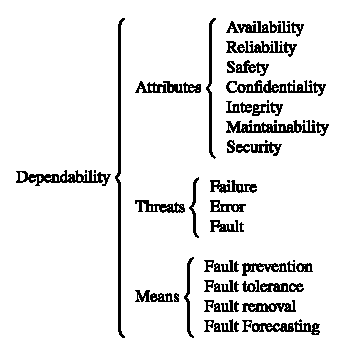
\includegraphics[width=0.3\textwidth]{imgs/div_avizienis}
\caption{Dependability systematic classification.}
\label{fig:div_avizienis}
\end{figure}

The first group is used to provide an analysis about the quality of a dependable
system. The second group brings the terms used to express undesirable threats --
but, in principle, not unexpected -- that makes a system become not dependable.
Finally, the third group shows the means and the techniques by which it becomes
possible to offer a dependable service.

\begin{comment}
Tendo destacado tal divisão, deve-se esclarecer o significado da utilização dos
três termos que muitas vezes podem vir a ser confundidos: errors, faults and
failures.
\end{comment}

About the second group, the term {\it failure} must be used to indicate when
occur a system behavior deviation, making it incapable to provide the service
for which was designed. An {\it error}, however, is related to the system state
and can lead to a failure. Briefly, if there is an error, then exists a sequence
of actions that can be lead to a failure. Last but no least, the term {\it
fault} is the cause of an error and is related to a defect. Normally, it is said
that the term fault may be defined as a defect that has the potential to generate
errors.

\begin{comment}
Considerando que os sistemas reais são normalmente compostos por subsistemas, é
comum se observar que uma falha leva a um erro, que por sua vez pode levar a uma
avaria, podendo vir a gerar novas falhas e dar início a uma reação em cadeia,
tal como mostra a Fig \ref{fig:chain_reaction}.Contudo, nem sempre uma falha
conduz a um erro, assim como nem sempre um erro conduz a uma avaria, mas todos
os erros resultam de falhas e todas as avarias resultam de erros.

\begin{figure}[htb]
\centering
    
\includegraphics[width=0.65\textwidth]{imgs/chain_reaction}
    \caption{Chain reaction of faults, errors and failures.}
    \label{fig:chain_reaction}
\end{figure}
\end{comment}

\begin{comment}
% ------------------------------------------------------------------------------
\subsection{Fault types}
De acordo com \citet{silva:2008}, as falhas em um processo industrial podem ser
classificadas em relação a vários aspectos. Em se tratando da classificação
quanto ao tempo, as falhas podem ser abruptas, incipientes ou intermitentes, tal
como mostra a Fig \ref{fig:fault_types}.

\begin{figure}[htb]
\centering
    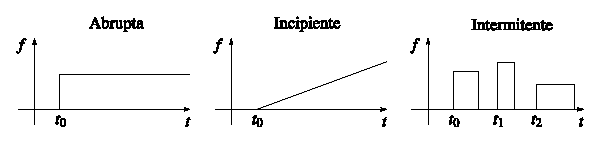
\includegraphics[width=0.65\textwidth]{imgs/fault_types}
    \caption{Características temporais das falhas quanto a sua persistência.}
    \label{fig:fault_types}
\end{figure}
\end{comment}

\begin{comment}
As falhas abruptas surgem repentinamente, podendo ser decorrentes de imprevistos
ou até mesmo de acidentes. Essas falhas mudam o comportamento do processo
rapidamente, exigindo contra-ações velozes e eficazes que possam minimizar as
consequências do ocorrido.

As falhas incipientes iniciam a partir de pequenos desvios comportamentais do
sistema, podendo ser mascaradas pelos controladores. Muitas vezes essas falhas
acabam passando despercebidas pelos operadores ou até mesmo pelos sistemas de
detecção e diagnóstico de falhas.

As falhas intermitentes são aquelas que ocorrem durante um certo período de
tempo e, em seguida, desaparecem, voltando a aparecer após um novo intervalo.
Podem ser causadas por alguma perturbação periódica ou por alguma situação que
se repita ciclicamente
\end{comment}

\begin{comment}
Com relação a localização das falhas, estas podem ocorrer nos sensores, nos
atuadores ou na estrutura do sistema \citep{silva:2008}. As falhas nos sensores
são observadas através de variações específicas nas medições, as quais podem ser
descaracterizadas como variações válidas do sistema. As falhas nos atuadores
podem ser vistas como qualquer mau funcionamento do equipamento que atua no
sistema. As falhas na estrutura, ou falhas estruturais, ocorrem quando alguma
alteração do sistema muda, de alguma forma, a relação original de entrada e
saída do processo ou quando ocorre algum problema com algum dos dispositivos,
desde que não sejam sensores ou atuadores, como por exemplo, os transmissores de
sinal. Considerando então um processo genérico, pode-se citar como exemplos de
falhas aquelas exibidas pela Tab. \ref{tab:gen_faults}.

\begin{table}[htb]
%\small
\centering
\caption{Exemplos de falhas para um processo genérico.}
\label{tab:gen_faults}
\begin{tabular}{|c|c|c|}
\hline
{\bf Sensores} & {\bf Atuadores} & {\bf Estrutura}\\
\hline
Erro de leitura & Erro de escrita & Erro de transmissão\\
\hline
Uncalibrated & Erro de leitura & Perda de comunicação\\
\hline
Sensibilidade à ruído & Sensibilidade à ruído & Sensibilidade a ruído
(transmissor)\\
\hline
Queima & Queima & Queima (transmissor)\\
\hline
- & Atraso de transporte & Atraso de propagação de sinais\\
\hline
\end{tabular}
\end{table}

\end{comment}
% ------------------------------------------------------------------------------
\subsection{Fault detection and diagnosis}
\begin{comment}
Considerando que os processos industrias estão se tornando cada vez mais
integrados e complexos, a ocorrência de falhas passa a ser mais um fator de
complicação. As falhas que antes poderiam ser detectadas facilmente por medições
diretas de determinada variável dependem agora de um conjunto de variáveis que
atuam simultaneamente no sistema
\end{comment}

In order to ensure the success of planned operations and recognize the
behaviorial problems in the process, many supervision and monitoring systems are
being developed. To \citet{chiang:2001}, among other functions, these systems
can detect, diagnose and eliminate faults, ensuring that the process operations
satisfies the performance specifications.

Additionally, the information provided by a monitoring system should not only
inform the system operator about what is going on, but also help him to take
corrective measures in order to remedy the problem. As a result, the ineffective
time will be reduced, the system protection will be increased and the
operational costs will be decreased.

\citet{chiang:2001} shows that there are four states involved in the process
monitoring: fault detection, fault isolation, fault diagnosis and fault
recovery, as shown in Fig. \ref{fig:states}.

\begin{figure}[htb]
\centering
    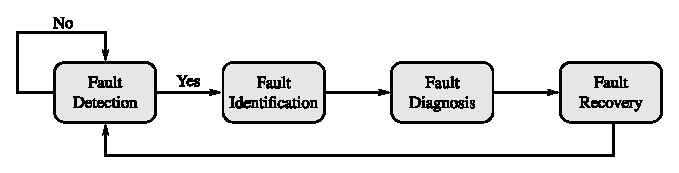
\includegraphics[width=0.6\textwidth]{imgs/states}
    \caption{States of fault detection and diagnosis.}
    \label{fig:states}
\end{figure}

Although arranged as a sequence of actions, all states are not always strictly
necessary. Often, automated changes from one state to another is transparent to
the operator, displaying only the crucial information to take appropriate action
\citep{chiang:2001}.

\begin{comment}
A detecção da falha determina se ocorreu ou não uma falha. Quando realizada de
maneira antecipada, a detecção de falhas pode fornecer informações valiosas com
relação aos problemas que estão por acontecer. Assim, através de ações
apropriadas, pode-se evitar grandes perturbações no processo.

A identificação da falha tem por objetivo identificar as variáveis mais
importantes para que se realize um diagnóstico apropriado. Para isso, essa fase
procura concentrar as atenções do operador nos subsistemas mais pertinentes à
falha, de tal modo que o efeito desta possa ser eliminado de maneira mais
eficiente.

A fase de diagnóstico da falha determina que falha ocorreu. De acordo com
\citet{isermann:2004}, essa fase deverá indicar o maior número de detalhes
possíveis a respeito da falha, tais como a intensidade, a localização e o
momento em que a falha foi detectada. Essa fase é considerada essencial para uma
contra-ação ou eliminação da falha.

Por fim, a fase de recuperação da falha, também conhecida como fase de
intervenção, tem por objetivo remover o efeito da falha para com o sistema,
dando início a um novo ciclo de detecção e diagnóstico.

% ------------------------------------------------------------------------------
\subsection{Neural networks for detection and diagnosis}
Com a introdução das novas tecnologias de medição e o consequente aumento do
número de instrumentos nos processos industrias, o número de informações
disponíveis para um dado sistema tornou-se demasiadamente grande. Tal situação
acaba por aumentar ainda mais a complexidade de processamento, tendo em vista
que cada vez mais os procedimentos de DDF utilizam dados de histórico do
processo. Dentre os exemplos desses métodos que fazem uso de histórico do
processo estão aqueles são baseados em RNAs.

Unindo essas características com aquelas expostas no Cap. 2, serão utilizadas
nesse trabalho duas estruturas neurais com o objetivo de identificar o processo
de estudo de caso e realizar a detecção e o diagnóstico de falhas a partir de
seu histórico.  As estruturas propostas serão apresentadas na seção seguinte,
após a descrição do modelo de estudo de caso.
\end{comment}

% ==============================================================================
% PROPOSED SYSTEM
% ==============================================================================
\section{PROPOSED SYSTEM}\label{sec:proposed}
\begin{comment}
Existem diversos métodos consolidados para detecção e isolamento de falhas,
sendo alguns deles baseados em redundância física de componentes de hardware,
como sensores, atuadores e controladores. Entretanto, a duplicação de
componentes de hardware nem sempre é possível, uma vez que os custos
relacionados com a adição de novos componentes podem elevar o orçamento
demasiadamente.

Devido a esse elevado custo, existe uma fronteira clara e inerente à aplicação
de técnicas de tolerância a falhas. A escolha adequada dos dispositivos físicos
e dos softwares devem levar em consideração as exigências específicas de cada
sistema, de tal maneira que se possa contornar o custo associado ao emprego
dessas técnicas \citep{weber:2002}.
\end{comment}

% ------------------------------------------------------------------------------
\subsection{Case study}
At the end of the introductory section, this paper proposes a system development
for FDD in a dynamic process. The process in question consists of a coupled tank
system developed by Quanser\reg, schematically represented in Fig.
\ref{fig:tanks}.

\begin{figure}[htb]
\centering
\subfigure[Original configuration.]
{
    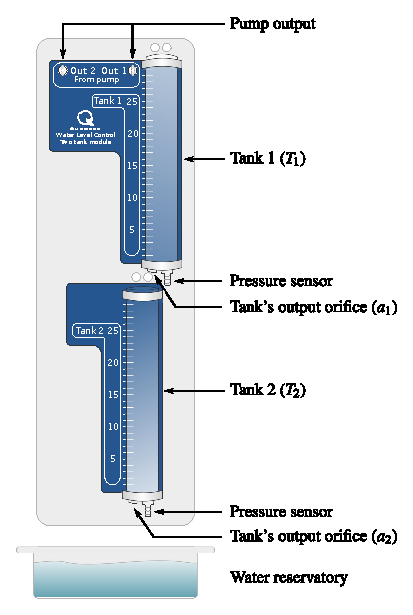
\includegraphics[height=225px]{imgs/tanks}
    \label{fig:tanks}
}
\qquad
\subfigure[Proposed configuration.]
{
    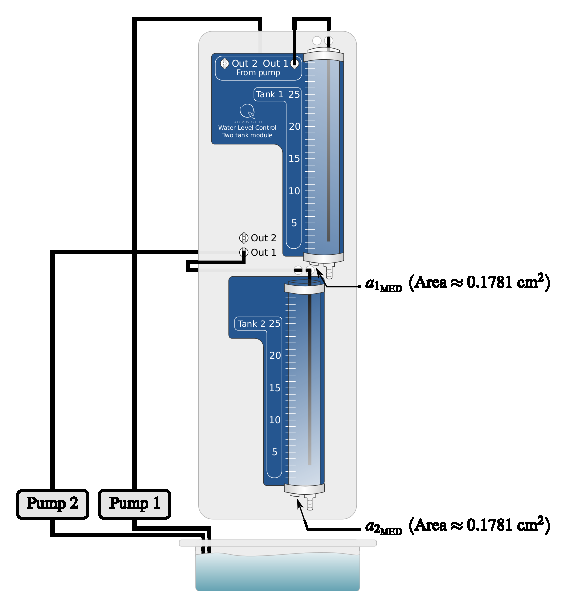
\includegraphics[height=225px]{imgs/new_config}
    \label{fig:new_config}
}
    \caption{Case study -- Coupled Water Tanks.}
\end{figure}

\begin{comment}
O sistema original consiste de uma bomba de água de corrente contínua e dois
tanques acoplados. A alimentação de água pela bomba se dá de forma vertical
através de dois orifícios com conectores normalmente fechados, de diferentes
diâmetros, denominados Out 1 e Out 2. Para facilitar o entendimento e evitar
confusões com relação aos orifícios de saída dos tanques (a1 e a2), esses
orifícios serão tratados como orifícios de entrada
\end{comment}

The tanks ($T_1$ e $T_2$) are mounted on the front of the support base and
positioned in such way that the water flows from the upper tank ($T_1$) to the
bottom tank ($T_2$) through orifice $a_1$, and from the $T_2$ to the water
reservatory through orifice $a_2$. The output water flow varies according to the
orifices $a_1$ and $a_2$, available in three different diameters.

\begin{comment}
% ------------------------------------------------------------------------------
\subsection{Mathematical model of a coupled water tanks} 
\end{comment}
Since the two tanks have the same cross-sectional area ($A_1 = A_2$), their
dynamics are similar. However, find a mathematical model that adequately
describes the dynamics of such tanks is not so simple, because the general
equations of motion and energy that describe the fluid flow are quite
complicated. Therefore, some fundamental assumptions are needed. So, it is
assumed that the water in the tank is incompressible and the flow is
non-viscous, non-rotational and regular \citep{dorf:2009}. Considering these
aspects, after a series of algebraic manipulations using Bernoulli's equation,
the equations of the model for a direct feed in $T_1$, can be described by Eqs.
(\ref{eq:l1_ponto}) and (\ref{eq:l2_ponto}).

\begin{eqnarray}
\dot{L_1} & = & \frac{K_m}{A}V_p -
                \left[\frac{a_1}{A}\sqrt{2g}\right]\sqrt{L_1}
                \label{eq:l1_ponto}\\
\dot{L_2} & = & \left[\frac{a_1}{A}\sqrt{2g}\right]\sqrt{L_1} -
                \left[\frac{a_2}{A}\sqrt{2g}\right]\sqrt{L_2}
                \label{eq:l2_ponto}
\end{eqnarray}
%
where $K_m$ represents the pump flow constant, $V_p$ the voltage applied to the
pump, $a_i$ the $T_i$'s output orifice, $L_i$ the water level in $T_i$ and $g$
the gravity acceleration.

In order to make the proposed system more generic and possibly make further
studies on fault tolerance, the coupled tank system was modified by introducing
another pump with the same characteristics as the first, as shown in Fig.
\ref{fig:new_config}.
É evidente que, nesse caso, o sistema deixa de ser SISO e passa a ser MIMO. Por
esse motivo, esse sistema será o utilizado como modelo de estudo de caso no
trabalho. A única modificação existente nas equações que regem a dinâmica do
modelo é a introdução de uma nova variável na equação do segundo tanque, em
virtude da adição da segunda bomba. Assim, as equações finais do modelo de
estudo de caso serão:

\begin{eqnarray}
\dot{L_1} & = & \frac{K_m}{A}V_{p_{\tiny 1}} -
                \left[\frac{a_1}{A}\sqrt{2g}\right]\sqrt{L_1}
                \label{eq:l1_ponto_fin}\\
\dot{L_2} & = & \frac{K_m}{A}V_{p_{\tiny 2}} +
                \left[\frac{a_1}{A}\sqrt{2g}\right]\sqrt{L_1} -
                \left[\frac{a_2}{A}\sqrt{2g}\right]\sqrt{L_2}
                \label{eq:l2_ponto_fin}
\end{eqnarray}
%
em que $V_{p_{\tiny 1}}$ se refere à tensão aplicada na Bomba 1 ($B_1$) e
$V_{p_{\tiny 2}}$ à tensão aplicada na Bomba 2 ($B_2$).

% ------------------------------------------------------------------------------
\subsection{Simulated faults}
Apesar das diversas falhas que podem vir a existir em um sistema tanques
acoplados, somente algumas destas foram selecionadas para serem simuladas,
conforme Tab. \ref{tab:faults}.

\begin{table}[!htb]
\centering
\caption{Selected faults -- Classification.}
\label{tab:faults}
\begin{tabular}{|c|c|}
\hline
{\bf Name} & {\bf Acronym}\\
\hline
\multicolumn{2}{|l|}{\bf Sensors}\\
\hline
Uncalibrated Gain & UGSeF\\
\hline
Uncalibrated Offset & UOSeF\\
\hline
Noise Sensitivity & NSSeF\\
\hline
Burned Sensor & BSeF\\
\hline
\multicolumn{2}{|l|}{\bf Actuators}\\
\hline
Uncalibrated Gain & UGAF\\
\hline
Uncalibrated Offset & UOAF\\
\hline
Noise Sensitivity & NSAF\\
\hline
$K_m$ variation & $K_m$AF\\
\hline
Burned Actuator & BAF\\
\hline
\multicolumn{2}{|l|}{\bf Structural}\\
\hline
Tank's Leak & TLStF\\
\hline
Tank's $a_i$ variation & T$a_i$VStF\\
\hline
Tank's $a_i$ obstruction & T$a_i$OStF\\
\hline
\end{tabular}
\end{table}

Nesses tipos de simulação é comum expor todo o sistema à situações adversas, não
comumente presentes no dia a dia, o que pode vir a causar danos em toda a
estrutura envolvida. Sendo assim, optou-se por simular computacionalmente o
modelo do sistema, evitando assim qualquer problema relacionado à queima dos
dispositivos.

\begin{comment}
Para dar mais liberdade de configuração à simulação, todo o sistema foi
desenvolvido em C++, através do método de Runge-Kutta de 4\textordfeminine\
ordem, permitindo que os parâmetros das falhas a serem simuladas fossem
modificados a partir de um arquivo de texto. 
\end{comment}

\begin{comment}
A Fig. \ref{fig:screenshot} mostra uma captura de tela do sistema em
funcionamento.

\begin{figure}[htb]
\centering
    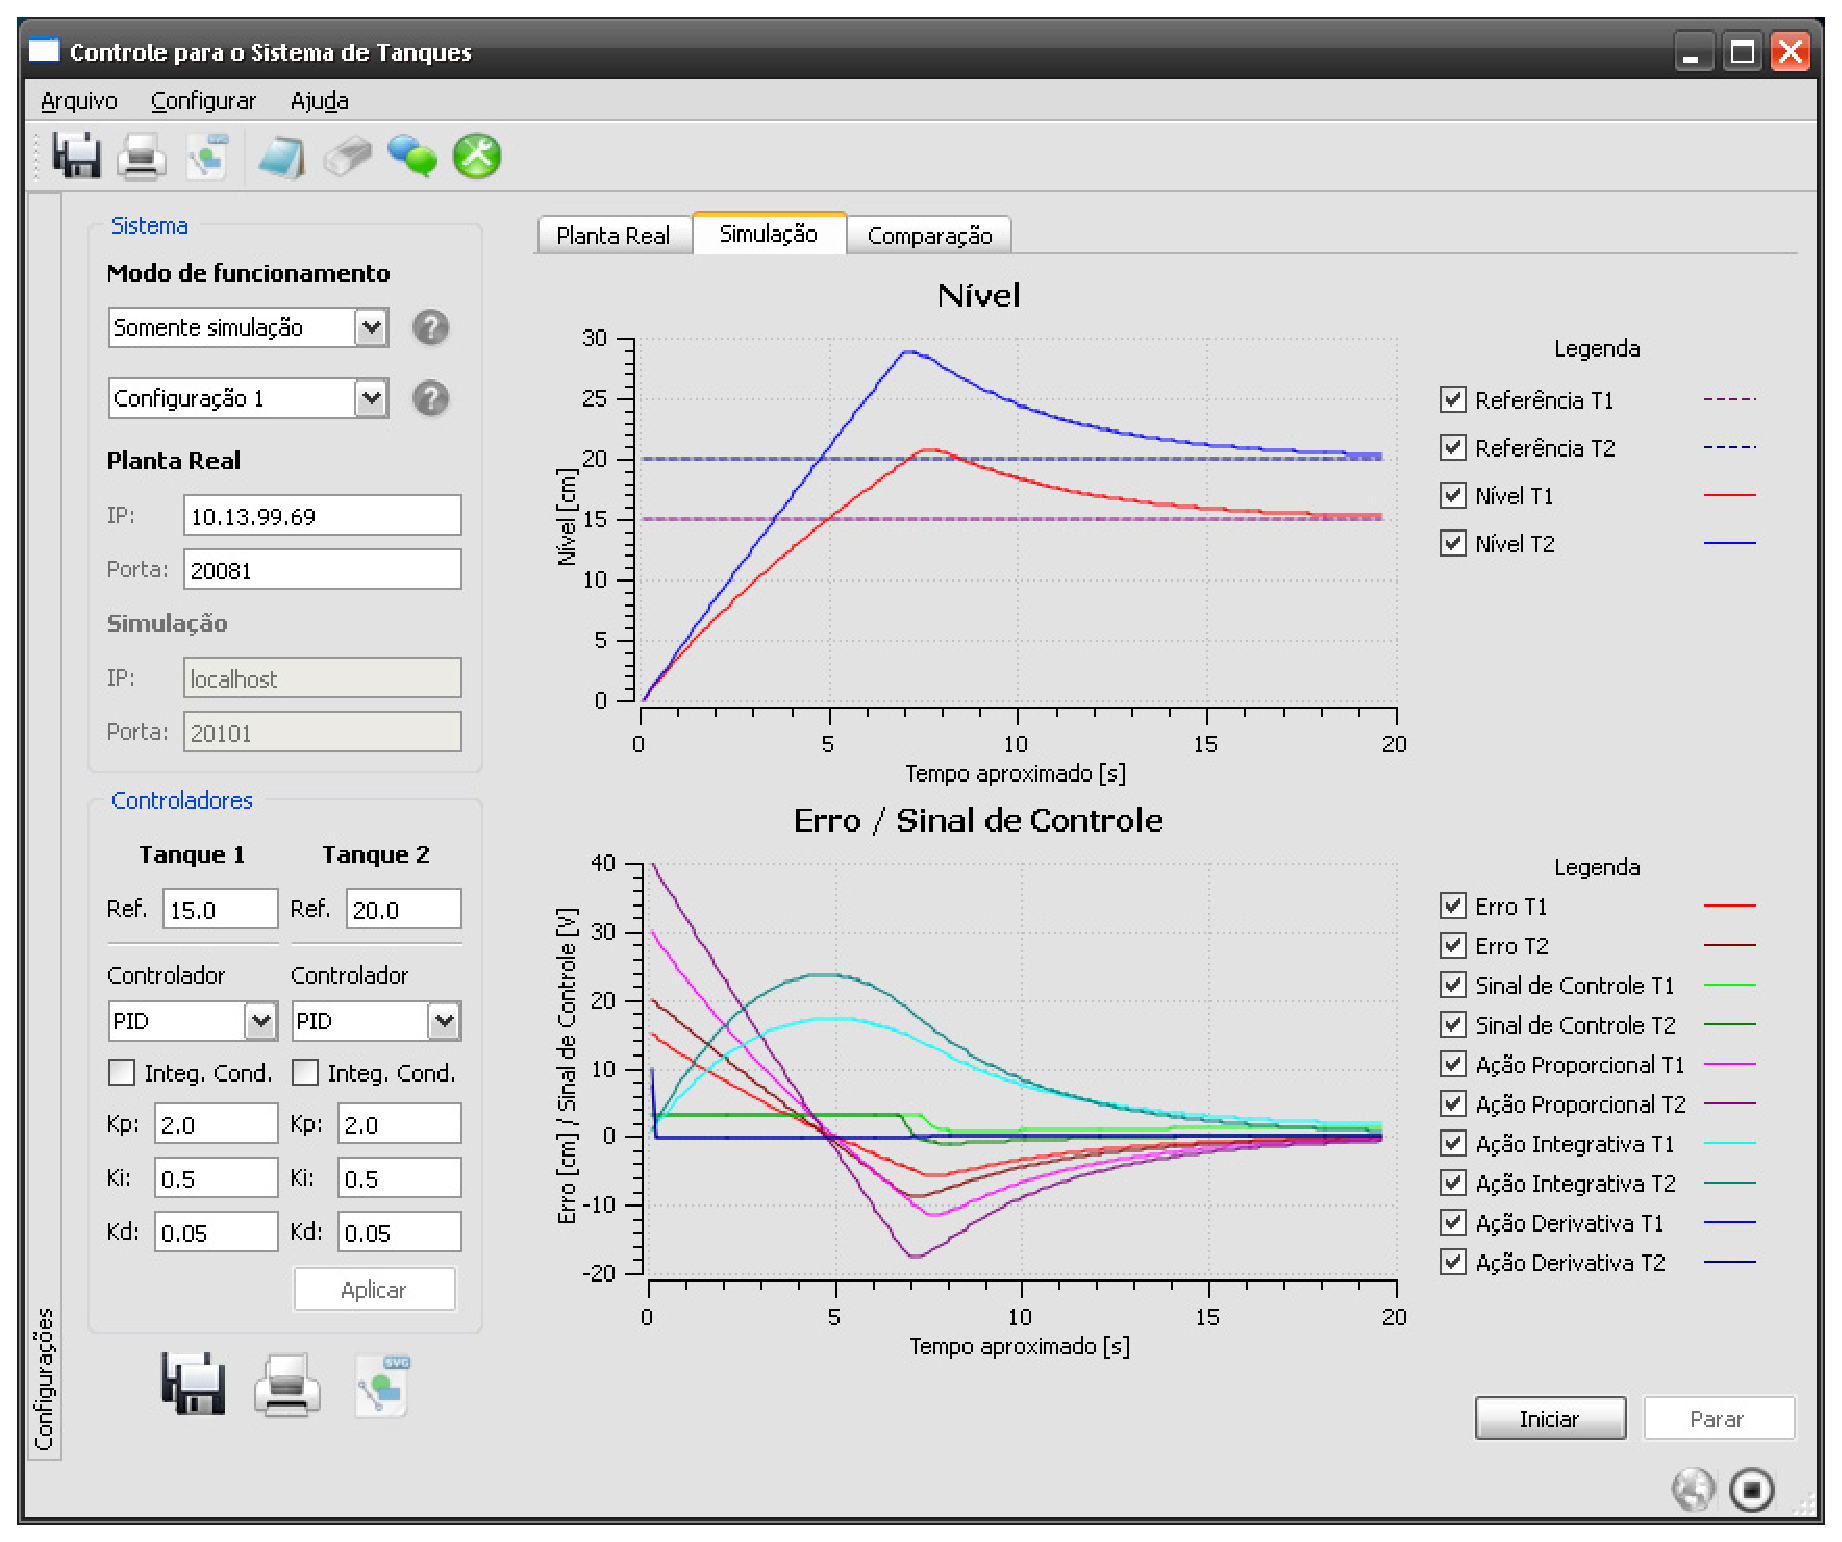
\includegraphics[width=0.6\textwidth]{imgs/screenshot}
    \caption{A screenshot from the developed system.}
    \label{fig:screenshot}
\end{figure}
\end{comment}

\begin{comment}
Nesse sistema, cada um dos parâmetros do arquivo de entrada deveria ser
especificado em uma coluna e o número de linhas equivale ao número de amostras a
serem simuladas. O período de amostragem utilizado na simulação do sistema é de
100 (cem) milissegundos, o mesmo utilizado para o controle da planta real.

Além disso, o sistema implementa as rotinas de dois controladores que podem ser
configurados para operarem como controladores P, PI, PD, PID ou PI-D. Os ganhos
pro porcionais, integrais e derivativos são introduzidos na interface do
usuário. 

Esse mesmo sistema pode ainda ser utilizado para operar com a planta real,
fazendo aquisições dos dados através da rede (local ou remota), utilizando
sockets TCP, se comunicando com um servidor implementado conforme mostrado em
Oliveira (2008). A configuração do endereço IP e da porta de comunicação também
é realizada a partir da interface do usuário. 
\end{comment}

% ------------------------------------------------------------------------------
\subsection{Selected neural structures}
Tanto para a identificação do modelo quanto para a detecção e o diagnóstico das
falhas, deve-se ter bastante cuidado ao se escolher a estrutura e a arquitetura
das redes neurais. Em ambos os casos, uma escolha inadequada pode fazer com que
o sistema não se comporte de maneira adequada e não realize a função para o qual
foi designado.

% ------------------------------------------------------------------------------
\subsubsection{Neural network for model identification}
A estrutura neural de identificação busca representar a dinâmica do sistema de
tanques através de uma única rede neural, a qual receberia como entrada os
valores passados dos níveis, $L_1(k-1)$ e $L_2(k-1)$, e os valores de tensão
aplicados, $V_{p_{\tiny 1}}(k-1)$ e $V_{p_{\tiny 2}}(k-1)$, gerando uma
estimativa dos níveis em sua saída, denominadas $\widehat{L}_1(k)$ e b
$\widehat{L}_2(k)$. A Fig. \ref{fig:ann_id} representa um diagrama esquemático
do funcionamento dessa primeira proposta.

\begin{figure}[htb]
\centering
    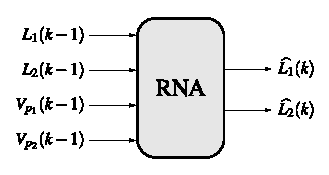
\includegraphics[width=0.3\textwidth]{imgs/ann_id}
    \caption{Neural network structure for model identification.}
    \label{fig:ann_id}
\end{figure}

A melhor rede neural treinada para esse propósito foi obtida a partir de um
modelo NNARX de segunda ordem, com oito neurônios na camada oculta. O erro médio
quadrático de estimativa foi de $3.73 \times 10^{-6}$.

% ------------------------------------------------------------------------------
\subsubsection{Neural network for fault detection and diagnosis}
A estrutura de DDF foi composta por várias redes neurais, em que cada uma destas
está associada a uma única falha, formando um conjunto de redes
``especialistas''. Não se trata, entretanto, de uma máquina de comitê de
especialistas, uma vez que não existe uma rede que realiza a tomada de decisões.

A entrada de cada uma das redes é composta pelos valores passados dos níveis,
$L_1(k-1)$ e $L_2(k-1)$, das tensões, $V_{p_{\tiny 1}}(k-1)$ e $V_{p_{\tiny
2}}(k-1)$, e pelos erros residuais produzidos a partir da diferença entre o
nível real e o nível estimado pela rede $e_i(k) = L_i(k) - \widehat{L}_i(k)$. Já
a saída de cada rede é composta por uma palavra binária de 2 bits, a qual indica
se aquela falha está sendo detectada em $T_1$ em $T_2$ ou em $T_1$ e $T_2$
simultaneamente. A Fig. \ref{fig:ann_fdd} representa um diagrama esquemático
dessa proposta.

\begin{figure}[htb]
\centering
    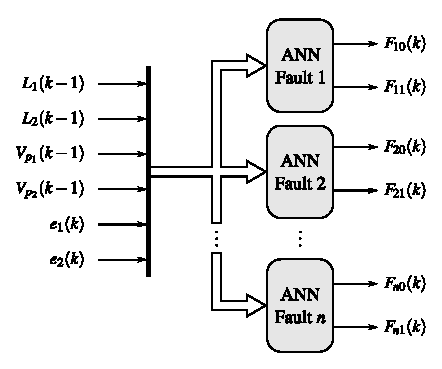
\includegraphics[width=0.4\textwidth]{imgs/ann_fdd}
    \caption{Neural network structure for fault detection and diagnosis.}
    \label{fig:ann_fdd}
\end{figure}

A opção por esse tipo desarticulado de redes neurais se dá por diversos fatores.
Um ponto que se pode destacar é o fato de que mais de uma falha pode estar
acontecendo simultaneamente no sistema. Nesse caso, se fosse utilizada apenas
uma estrutura neural, gerando $N$ palavras distintas na saída (uma para cada
falha), seria necessário também estabelecer valores de saída para todas as
combinações de falhas possíveis, pois estas também deveriam ser representadas
nas $N$ possíveis palavras.  Considerando somente as doze falhas selecionadas,
tomadas duas a duas, teria-se um total de 66 possíveis combinações a serem
geradas. Se todas as combinações fossem consideradas esse número cresceria de
maneira exorbitante.

Com essa configuração, diversos tipos de redes podem ser utilizadas para cada
uma das falhas o que pode vir a aumentar a eficiência do sistema de detecção.
Além disso, a modificação da estrutura de detecção de uma falha não
irá influenciar em nenhuma outra. Ou seja, se em determinado momento for
percebido que a introdução de uma nova variável faz com que uma das falhas seja
detectada de maneira mais rápida ou eficiente, apenas aquela rede neural
precisará ser novamente treinada.

Tendo conhecido todos os subsistemas a serem utilizados, pode-se observar na
Fig. \ref{fig:comp} a estrutura do sistema de DDF proposto.

\begin{figure}[htb]
\centering
    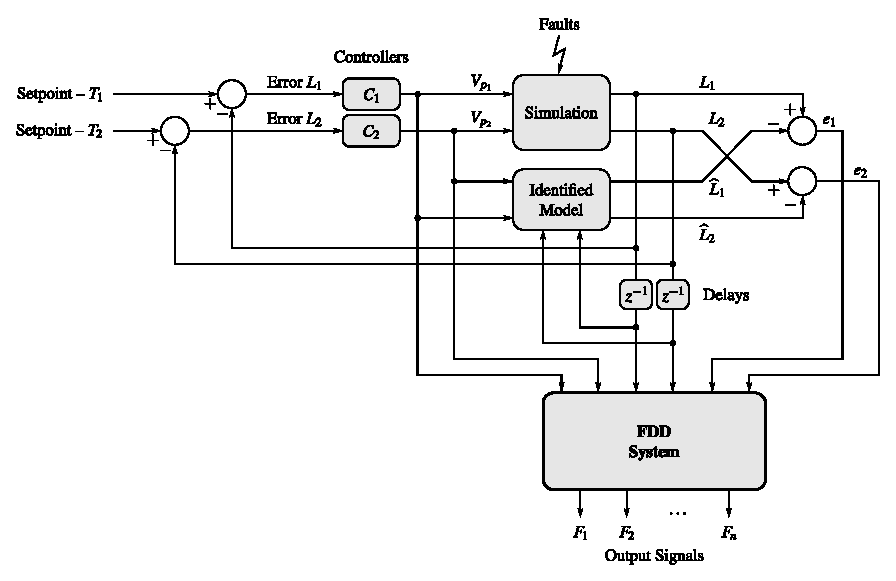
\includegraphics[width=0.75\textwidth]{imgs/comp}
    \caption{Schematic diagram of system composition.}
    \label{fig:comp}
\end{figure}

Acoplar tal sistema à um ambiente de monitoramento e supervisão, ou ainda
associá-lo à técnicas de controle tolerante à falhas, consiste simplesmente em
processar as informações disponíveis na interface de saída do módulo de DDF.
Contudo, isso não faz parte do escopo deste trabalho.

% ==============================================================================
% RESULTS
% ==============================================================================
\section{RESULTS}\label{sec:results}

% ------------------------------------------------------------------------------
\subsection{Data acquisition}
Tanto para o processo de identificação quanto para o processo de detecção, o
primeiro passo a ser dado é a obtenção das amostras experimentais para o
treinamento supervisionado das redes neurais de identificação do modelo e de
detecção e diagnóstico das falhas.

Dessa maneira, realizou-se a coleta dos dados a partir da estimulação do sistema
simulado através da aplicação de sinais binários pseudo aleatórios (Pseudo
Random Binary Signals -- PRBS) à referência de cada um dos tanques e aos
parâmetros do sistema que simulam as falhas

Para a identificação, a faixa de valores aplicados se deu do nível mínimo (zero)
ao máximo (trinta). Já para a detecção das falhas, os valores foram aplicados
conforme Tab. \ref{tab:values}. Nessa tabela, os valores gerados no intervalo
determinado pelos mínimos e máximos de cada parâmetro eram multiplicados pelos
respectivos valores padrão e aplicados ao modelo. Perceba que nas falhas dos
atuadores, as tensões a serem aplicadas podem vir a danificar a bomba. Por esse
motivo não seria viável obter as amostras do processo real, mas sim a partir de
uma simulação.

\begin{table}[htb]
\small
\caption{Applied values for training step.}
\label{tab:values}
\centering
\begin{threeparttable}
\begin{tabular}{|c|c|c|c|c|}
\hline
{\bf Fault} & {\bf Default value} & {\bf Min} & {\bf Max} & 
{\bf Representativeness}\\
\hline
UGSeF & 0,16\tnote{$*$} & 
0,8 & 1,2 & Up to $\pm 6$ cm\\
\hline
UOSeF & 1,0 & -3,0 & 3,0 & Up to $\pm 3$ cm\\
\hline
NSSeF & 1,0 & -0,03 & 0,03 & Up to $\pm 9$ cm\\
\hline
BSeF & 1,0 & 0,0 & 0,0 & -- \\
\hline
UGAF & 1,0 & 0,8 & 1,0 & Up to -3 Volts\\
\hline
UOAF & 1,0 & -1,0 & 0,0 & Up to -1 Volts\\
\hline
NSAF & 1,0 & -0,03 & 0,03 & Up to $\pm 0,45$ Volts\\
\hline
$K_m$AF & $K_m$ & 0,7 & 1,1 & --\\
\hline
BAF & 1,0 & 0,0 & 0,0 & --\\
\hline
TLStF & $a_{i_{\text{\tiny MED}}}$ & 
0,25 & 0,75 & 25 a 75\% de $a_{i_{\text{\tiny MED}}}$\\
\hline
T$a_i$VStF & $a_{i_{\text{\tiny MED}}}$ & 
0,75 & 1,25 & $\pm 25\%$ de $a_{i_{\text{\tiny MED}}}$\\
\hline
T$a_i$OStF & $a_{i_{\text{\tiny MED}}}$ & 
0,0 & 0,5 & --\\
\hline
\end{tabular}
\begin{tablenotes}
\item [$*$] Established by the manufacturer.
\end{tablenotes}
\end{threeparttable}
\end{table}

Os sinais pseudo aleatórios gerados se mantiveram dentro dos limites
estabelecidos durante todo o tempo da simulação. Para o processo de
identificação foram obtidas 6000 (seis mil) amostras, equivalentes à 10 (dez)
minutos de simulação. Já para a detecção o processo foi simulado durante 20
(vinte) minutos, o que correspondeu a obtenção de 12000 (doze mil) amostras.
Todos os dados foram coletados com um período de amostragem de 100 ms, idêntico
ao utilizado na planta real.

De posse dos valores obtidos, iniciou-se a fase de treinamento das RNAs. Todas
as redes foram treinadas de modo offline com o toolbox de redes neurais do
software matemático Matlab\reg, utilizando o algoritmo LMA. Ao final de cada etapa
de treinamento as redes eram submetidas aos testes de validação com o intuito de
avaliar suas capacidades de generalização.

% ------------------------------------------------------------------------------
\subsection{Selected neural networks}
Como já foi visto, a melhor rede utilizada para a identificação do modelo foi
obtida a partir de uma estrutura NNARX de segunda ordem com oito neurônios na
camada oculta. Essa rede foi selecionada dentre outras 54 que haviam sido
treinadas para esta mesma finalidade.

Para o processo de detecção e diagnóstico das falhas, o número de redes neurais
treinadas aumenta de maneira significativa. Para cada ordem da estrutura NNARX
selecionada, o número de neurônios na camada oculta era modificado três vezes.
Cada vez que esse número era modificado, eram treinadas seis redes neurais., o
que garantia que as redes selecionadas não seriam comprometidas por problemas de
não convergência devido à uma má inicialização dos pesos ou devido à mínimos
locais. Dessa forma, para uma estrutura de segunda ordem, por exemplo, eram
treinadas $3 \times 6 = 18$ redes neurais.  

Como foram selecionadas estruturas de segunda, terceira e quarta ordem, o número
de redes treinadas corresponderia a $18 \times 3 = 54$ para cada falha.
Entretanto, haviam doze falhas a serem treinadas. Assim, o número total foi de
$54 \times 12 = 648$ redes neurais distintas.

Devido a esse grande número, todas as redes passavam por um processo de
validação dividido em três simulações. Em cada simulação eram contabilizados os
Erros de Tipo I e os Erros de Tipo II, obtendo então uma média total de erros
para cada estrutura. Os valores obtidos durante o processo de seleção podem ser
observados na Tab. \ref{tab:best_ann}.

\begin{table}[htb]
\centering
\caption{Best ANNs for FDD.}
\label{tab:best_ann}
\begin{threeparttable}
\begin{tabular}{|c|c|c|c|c|c|c|c|}
\hline
\multirow{2}{*}{\bf Fault} &
\multirow{2}{*}{\bf Order} &
\multirow{2}{*}{{\bf HLN}\tnote{$*$}} &
\multirow{2}{*}{\bf Train. \#} &
{\bf Correct} & {\bf Type I} & {\bf Type II} & {\bf Total}\\
& & & & {\bf Answers} & {\bf Errors} & {\bf Errors} & {\bf Errors (\%)}\\
\hline
UGSeF & 4 & 28 & 2 & 23491,33 & 203,33 & 305,33 & 2,12\%\\
\hline
UOSeF & 4 & 28 & 5 & 23890,33 & 8,66 & 101 & 0,46\%\\
\hline
NSSeF & 4 & 20 & 3 & 23317 & 324,66 & 358,33 & 2,84\%\\
\hline
BSeF & 4 & 20 & 4 & 23994 & 0,66 & 5,33 & 0,02\%\\
\hline
UGAF & 2 & 8 & 3 & 20710,33 & 1626,66 & 1663 & 13,7\%\\
\hline
UOAF & 4 & 28 & 3 & 23075,33 & 635,66 & 289 & 3,85\%\\
\hline
{NSAF} & 2 & 8 & 6 & 14153,33 & 3407 & 6439,66 & 41,03\%\\
\hline
$K_m$AF & 2 & 8 & 5 & 20764,66 & 1551,33 & 1684 & 13,48\%\\
\hline
BAF & 4 & 28 & 6 & 23980 & 2,33 & 17,66 & 0,083\%\\
\hline
TLStF & 4 & 24 & 1 & 23774,33 & 74 & 151,66 & 0,94\%\\
\hline
T$a_i$VStF & 2 & 8 & 3 & 22465,33 & 437 & 1097,66 & 6,39\%\\
\hline
T$a_i$OStF & 2 & 12 & 4 & 23995,66 & 1 & 3,33 & 0,018\%\\
\hline
\end{tabular}
\begin{tablenotes}
\item [$*$] Hidden layer neurons.
\end{tablenotes}
\end{threeparttable}
\end{table}

Tendo selecionado a melhor estrutura de identificação e as melhores redes de
DDF, pôde-se compor o sistema e submetê-lo à simulação final de um minuto
e quarenta e cinco segundos, subdividida em intervalos de quinze segundos
conforme Fig. \ref{fig:intervals}.

\begin{figure}[htb]
\centering
    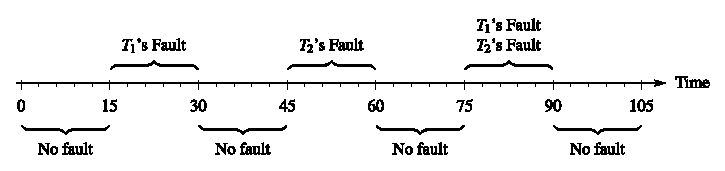
\includegraphics[width=0.6\textwidth]{imgs/intervals}
    \caption{Final simulation -- Intervals.}
    \label{fig:intervals}
\end{figure}

Nesta última validação, os valores de cada um dos parâmetros das falhas foram
mantidos fixos durante o intervalo em que aquela falha estava atuando no
sistema. Os valores utilizados em cada uma das doze simulações podem ser
observados na Tab. \ref{tab:used_val}.

\begin{table}[htb]
\centering
\caption{Used parameter values.}
\label{tab:used_val}
\begin{tabular}{|c|c|c|}
\hline
{\bf Simulação} & {\bf Falha} & {\bf Valor modificado}\\
\hline
1 & UGSeF & $\text{Gain} = 0,128$\\
\hline
2 & UOSeF & -2,0\ cm\\
\hline
3 & NSSeF & $\pm 2\%$\\
\hline
4 & BSeF & $\text{Gain} = 0,0$\\
\hline
5 & UGAF & $\text{Gain} = 0,8$\\
\hline
6 & UOAF & -0,5 Volts\\
\hline
7 & NSAF & $\pm 2\%$\\
\hline
8 & $K_m$AF & $K_m = 3,45$\\ 
\hline
9 & BAF & $\text{Gain} = 0,0$\\
\hline
10 & TLStF & $a_{\tiny VZ} = \frac{a_{\tiny MED}}{2}$\\
\hline
11 & T$a_i$VStF & $a_i = \frac{a_{\tiny MED}}{2}$\\
\hline
12 & T$a_i$OStF & ${a_i}' = \frac{a_{\tiny MED}}{4}$\\
\hline
\end{tabular}
\end{table}

% ------------------------------------------------------------------------------
\subsection{Obtained results}
Os resultados obtidos para cada uma das falhas podem ser vistos da Fig.
\ref{fig:fsedg} a \ref{fig:fsivros}. Nessas figuras, as áreas hachuradas em
vermelho representam os intervalos em que o sistema detectou a falha em $T_1$,
enquanto que as falhas hachuradas em azul representam os intervalos em que a
falha foi detectada em $T_2$.

A primeira falha a ser simulada foi a UGSeF, cujo resultado da detecção pode ser
observado na Fig. \ref{fig:fsedg}. Nessa simulação o valor do ganho do sensor
foi reduzido para 80\% do valor original. 

\begin{figure}[htb]
    \begin{minipage}[b]{0.48\linewidth}
        \scalebox{0.65}{% GNUPLOT: LaTeX picture with Postscript
\begingroup
  \makeatletter
  \providecommand\color[2][]{%
    \GenericError{(gnuplot) \space\space\space\@spaces}{%
      Package color not loaded in conjunction with
      terminal option `colourtext'%
    }{See the gnuplot documentation for explanation.%
    }{Either use 'blacktext' in gnuplot or load the package
      color.sty in LaTeX.}%
    \renewcommand\color[2][]{}%
  }%
  \providecommand\includegraphics[2][]{%
    \GenericError{(gnuplot) \space\space\space\@spaces}{%
      Package graphicx or graphics not loaded%
    }{See the gnuplot documentation for explanation.%
    }{The gnuplot epslatex terminal needs graphicx.sty or graphics.sty.}%
    \renewcommand\includegraphics[2][]{}%
  }%
  \providecommand\rotatebox[2]{#2}%
  \@ifundefined{ifGPcolor}{%
    \newif\ifGPcolor
    \GPcolortrue
  }{}%
  \@ifundefined{ifGPblacktext}{%
    \newif\ifGPblacktext
    \GPblacktexttrue
  }{}%
  % define a \g@addto@macro without @ in the name:
  \let\gplgaddtomacro\g@addto@macro
  % define empty templates for all commands taking text:
  \gdef\gplbacktext{}%
  \gdef\gplfronttext{}%
  \makeatother
  \ifGPblacktext
    % no textcolor at all
    \def\colorrgb#1{}%
    \def\colorgray#1{}%
  \else
    % gray or color?
    \ifGPcolor
      \def\colorrgb#1{\color[rgb]{#1}}%
      \def\colorgray#1{\color[gray]{#1}}%
      \expandafter\def\csname LTw\endcsname{\color{white}}%
      \expandafter\def\csname LTb\endcsname{\color{black}}%
      \expandafter\def\csname LTa\endcsname{\color{black}}%
      \expandafter\def\csname LT0\endcsname{\color[rgb]{1,0,0}}%
      \expandafter\def\csname LT1\endcsname{\color[rgb]{0,1,0}}%
      \expandafter\def\csname LT2\endcsname{\color[rgb]{0,0,1}}%
      \expandafter\def\csname LT3\endcsname{\color[rgb]{1,0,1}}%
      \expandafter\def\csname LT4\endcsname{\color[rgb]{0,1,1}}%
      \expandafter\def\csname LT5\endcsname{\color[rgb]{1,1,0}}%
      \expandafter\def\csname LT6\endcsname{\color[rgb]{0,0,0}}%
      \expandafter\def\csname LT7\endcsname{\color[rgb]{1,0.3,0}}%
      \expandafter\def\csname LT8\endcsname{\color[rgb]{0.5,0.5,0.5}}%
    \else
      % gray
      \def\colorrgb#1{\color{black}}%
      \def\colorgray#1{\color[gray]{#1}}%
      \expandafter\def\csname LTw\endcsname{\color{white}}%
      \expandafter\def\csname LTb\endcsname{\color{black}}%
      \expandafter\def\csname LTa\endcsname{\color{black}}%
      \expandafter\def\csname LT0\endcsname{\color{black}}%
      \expandafter\def\csname LT1\endcsname{\color{black}}%
      \expandafter\def\csname LT2\endcsname{\color{black}}%
      \expandafter\def\csname LT3\endcsname{\color{black}}%
      \expandafter\def\csname LT4\endcsname{\color{black}}%
      \expandafter\def\csname LT5\endcsname{\color{black}}%
      \expandafter\def\csname LT6\endcsname{\color{black}}%
      \expandafter\def\csname LT7\endcsname{\color{black}}%
      \expandafter\def\csname LT8\endcsname{\color{black}}%
    \fi
  \fi
  \setlength{\unitlength}{0.0500bp}%
  \begin{picture}(7200.00,5040.00)%
    \gplgaddtomacro\gplbacktext{%
      \csname LTb\endcsname%
      \put(726,3150){\makebox(0,0)[r]{\strut{} 5}}%
      \csname LTb\endcsname%
      \put(726,3780){\makebox(0,0)[r]{\strut{} 10}}%
      \csname LTb\endcsname%
      \put(726,4409){\makebox(0,0)[r]{\strut{} 15}}%
      \csname LTb\endcsname%
      \put(726,5039){\makebox(0,0)[r]{\strut{} 20}}%
      \csname LTb\endcsname%
      \put(921,2237){\makebox(0,0){\strut{}}}%
      \csname LTb\endcsname%
      \put(1771,2237){\makebox(0,0){\strut{}}}%
      \csname LTb\endcsname%
      \put(2620,2237){\makebox(0,0){\strut{}}}%
      \csname LTb\endcsname%
      \put(3470,2237){\makebox(0,0){\strut{}}}%
      \csname LTb\endcsname%
      \put(4320,2237){\makebox(0,0){\strut{}}}%
      \csname LTb\endcsname%
      \put(5170,2237){\makebox(0,0){\strut{}}}%
      \csname LTb\endcsname%
      \put(6019,2237){\makebox(0,0){\strut{}}}%
      \csname LTb\endcsname%
      \put(6869,2237){\makebox(0,0){\strut{}}}%
      \put(352,3779){\rotatebox{-270}{\makebox(0,0){\strut{}Nível [cm]}}}%
    }%
    \gplgaddtomacro\gplfronttext{%
      \csname LTb\endcsname%
      \put(6278,2913){\makebox(0,0)[r]{\strut{}Ref. $T_1$}}%
      \csname LTb\endcsname%
      \put(6278,2693){\makebox(0,0)[r]{\strut{}Saída $T_1$}}%
    }%
    \gplgaddtomacro\gplbacktext{%
      \csname LTb\endcsname%
      \put(726,0){\makebox(0,0)[r]{\strut{} 0}}%
      \csname LTb\endcsname%
      \put(726,420){\makebox(0,0)[r]{\strut{} 5}}%
      \csname LTb\endcsname%
      \put(726,840){\makebox(0,0)[r]{\strut{} 10}}%
      \csname LTb\endcsname%
      \put(726,1260){\makebox(0,0)[r]{\strut{} 15}}%
      \csname LTb\endcsname%
      \put(726,1680){\makebox(0,0)[r]{\strut{} 20}}%
      \csname LTb\endcsname%
      \put(726,2100){\makebox(0,0)[r]{\strut{} 25}}%
      \csname LTb\endcsname%
      \put(726,2520){\makebox(0,0)[r]{\strut{} 30}}%
      \csname LTb\endcsname%
      \put(921,-283){\makebox(0,0){\strut{}0}}%
      \csname LTb\endcsname%
      \put(1771,-283){\makebox(0,0){\strut{}15}}%
      \csname LTb\endcsname%
      \put(2620,-283){\makebox(0,0){\strut{}30}}%
      \csname LTb\endcsname%
      \put(3470,-283){\makebox(0,0){\strut{}45}}%
      \csname LTb\endcsname%
      \put(4320,-283){\makebox(0,0){\strut{}60}}%
      \csname LTb\endcsname%
      \put(5170,-283){\makebox(0,0){\strut{}75}}%
      \csname LTb\endcsname%
      \put(6019,-283){\makebox(0,0){\strut{}90}}%
      \csname LTb\endcsname%
      \put(6869,-283){\makebox(0,0){\strut{}105}}%
      \put(352,1260){\rotatebox{-270}{\makebox(0,0){\strut{}Nível [cm]}}}%
      \put(3895,-613){\makebox(0,0){\strut{}Tempo [s]}}%
    }%
    \gplgaddtomacro\gplfronttext{%
      \csname LTb\endcsname%
      \put(6278,393){\makebox(0,0)[r]{\strut{}Ref. $T_2$}}%
      \csname LTb\endcsname%
      \put(6278,173){\makebox(0,0)[r]{\strut{}Saída $T_2$}}%
    }%
    \gplbacktext
    \put(0,0){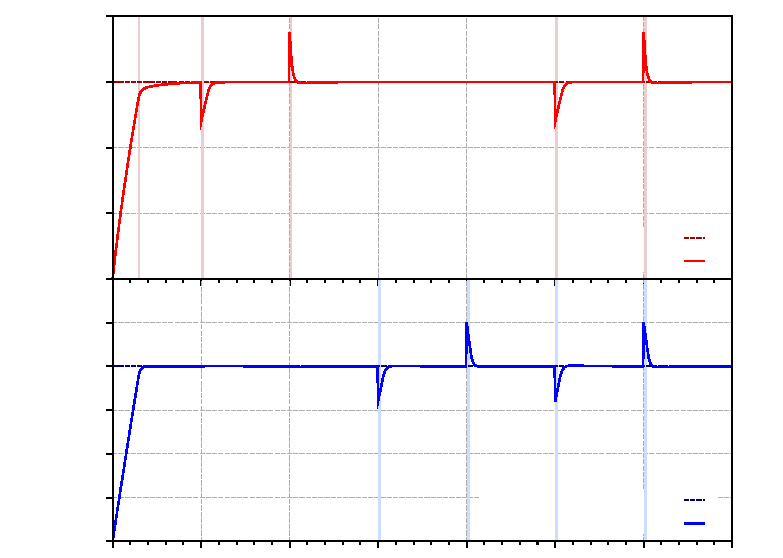
\includegraphics{fsedg}}%
    \gplfronttext
  \end{picture}%
\endgroup
}
        \vspace{0.5cm}
        \caption{UGSeF}
        \label{fig:fsedg}
    \end{minipage}
    \hfill
    \begin{minipage}[b]{0.48\linewidth}
        \scalebox{0.65}{% GNUPLOT: LaTeX picture with Postscript
\begingroup
  \makeatletter
  \providecommand\color[2][]{%
    \GenericError{(gnuplot) \space\space\space\@spaces}{%
      Package color not loaded in conjunction with
      terminal option `colourtext'%
    }{See the gnuplot documentation for explanation.%
    }{Either use 'blacktext' in gnuplot or load the package
      color.sty in LaTeX.}%
    \renewcommand\color[2][]{}%
  }%
  \providecommand\includegraphics[2][]{%
    \GenericError{(gnuplot) \space\space\space\@spaces}{%
      Package graphicx or graphics not loaded%
    }{See the gnuplot documentation for explanation.%
    }{The gnuplot epslatex terminal needs graphicx.sty or graphics.sty.}%
    \renewcommand\includegraphics[2][]{}%
  }%
  \providecommand\rotatebox[2]{#2}%
  \@ifundefined{ifGPcolor}{%
    \newif\ifGPcolor
    \GPcolortrue
  }{}%
  \@ifundefined{ifGPblacktext}{%
    \newif\ifGPblacktext
    \GPblacktexttrue
  }{}%
  % define a \g@addto@macro without @ in the name:
  \let\gplgaddtomacro\g@addto@macro
  % define empty templates for all commands taking text:
  \gdef\gplbacktext{}%
  \gdef\gplfronttext{}%
  \makeatother
  \ifGPblacktext
    % no textcolor at all
    \def\colorrgb#1{}%
    \def\colorgray#1{}%
  \else
    % gray or color?
    \ifGPcolor
      \def\colorrgb#1{\color[rgb]{#1}}%
      \def\colorgray#1{\color[gray]{#1}}%
      \expandafter\def\csname LTw\endcsname{\color{white}}%
      \expandafter\def\csname LTb\endcsname{\color{black}}%
      \expandafter\def\csname LTa\endcsname{\color{black}}%
      \expandafter\def\csname LT0\endcsname{\color[rgb]{1,0,0}}%
      \expandafter\def\csname LT1\endcsname{\color[rgb]{0,1,0}}%
      \expandafter\def\csname LT2\endcsname{\color[rgb]{0,0,1}}%
      \expandafter\def\csname LT3\endcsname{\color[rgb]{1,0,1}}%
      \expandafter\def\csname LT4\endcsname{\color[rgb]{0,1,1}}%
      \expandafter\def\csname LT5\endcsname{\color[rgb]{1,1,0}}%
      \expandafter\def\csname LT6\endcsname{\color[rgb]{0,0,0}}%
      \expandafter\def\csname LT7\endcsname{\color[rgb]{1,0.3,0}}%
      \expandafter\def\csname LT8\endcsname{\color[rgb]{0.5,0.5,0.5}}%
    \else
      % gray
      \def\colorrgb#1{\color{black}}%
      \def\colorgray#1{\color[gray]{#1}}%
      \expandafter\def\csname LTw\endcsname{\color{white}}%
      \expandafter\def\csname LTb\endcsname{\color{black}}%
      \expandafter\def\csname LTa\endcsname{\color{black}}%
      \expandafter\def\csname LT0\endcsname{\color{black}}%
      \expandafter\def\csname LT1\endcsname{\color{black}}%
      \expandafter\def\csname LT2\endcsname{\color{black}}%
      \expandafter\def\csname LT3\endcsname{\color{black}}%
      \expandafter\def\csname LT4\endcsname{\color{black}}%
      \expandafter\def\csname LT5\endcsname{\color{black}}%
      \expandafter\def\csname LT6\endcsname{\color{black}}%
      \expandafter\def\csname LT7\endcsname{\color{black}}%
      \expandafter\def\csname LT8\endcsname{\color{black}}%
    \fi
  \fi
  \setlength{\unitlength}{0.0500bp}%
  \begin{picture}(7200.00,5040.00)%
    \gplgaddtomacro\gplbacktext{%
      \csname LTb\endcsname%
      \put(726,3150){\makebox(0,0)[r]{\strut{} 5}}%
      \csname LTb\endcsname%
      \put(726,3780){\makebox(0,0)[r]{\strut{} 10}}%
      \csname LTb\endcsname%
      \put(726,4409){\makebox(0,0)[r]{\strut{} 15}}%
      \csname LTb\endcsname%
      \put(726,5039){\makebox(0,0)[r]{\strut{} 20}}%
      \csname LTb\endcsname%
      \put(921,2237){\makebox(0,0){\strut{}}}%
      \csname LTb\endcsname%
      \put(1771,2237){\makebox(0,0){\strut{}}}%
      \csname LTb\endcsname%
      \put(2620,2237){\makebox(0,0){\strut{}}}%
      \csname LTb\endcsname%
      \put(3470,2237){\makebox(0,0){\strut{}}}%
      \csname LTb\endcsname%
      \put(4320,2237){\makebox(0,0){\strut{}}}%
      \csname LTb\endcsname%
      \put(5170,2237){\makebox(0,0){\strut{}}}%
      \csname LTb\endcsname%
      \put(6019,2237){\makebox(0,0){\strut{}}}%
      \csname LTb\endcsname%
      \put(6869,2237){\makebox(0,0){\strut{}}}%
      \put(352,3779){\rotatebox{-270}{\makebox(0,0){\strut{}Level [cm]}}}%
    }%
    \gplgaddtomacro\gplfronttext{%
      \csname LTb\endcsname%
      \put(6278,2913){\makebox(0,0)[r]{\strut{}Setpoint $T_1$}}%
      \csname LTb\endcsname%
      \put(6278,2693){\makebox(0,0)[r]{\strut{}Output $T_1$}}%
    }%
    \gplgaddtomacro\gplbacktext{%
      \csname LTb\endcsname%
      \put(726,0){\makebox(0,0)[r]{\strut{} 0}}%
      \csname LTb\endcsname%
      \put(726,504){\makebox(0,0)[r]{\strut{} 5}}%
      \csname LTb\endcsname%
      \put(726,1008){\makebox(0,0)[r]{\strut{} 10}}%
      \csname LTb\endcsname%
      \put(726,1512){\makebox(0,0)[r]{\strut{} 15}}%
      \csname LTb\endcsname%
      \put(726,2016){\makebox(0,0)[r]{\strut{} 20}}%
      \csname LTb\endcsname%
      \put(726,2520){\makebox(0,0)[r]{\strut{} 25}}%
      \csname LTb\endcsname%
      \put(921,-283){\makebox(0,0){\strut{}0}}%
      \csname LTb\endcsname%
      \put(1771,-283){\makebox(0,0){\strut{}15}}%
      \csname LTb\endcsname%
      \put(2620,-283){\makebox(0,0){\strut{}30}}%
      \csname LTb\endcsname%
      \put(3470,-283){\makebox(0,0){\strut{}45}}%
      \csname LTb\endcsname%
      \put(4320,-283){\makebox(0,0){\strut{}60}}%
      \csname LTb\endcsname%
      \put(5170,-283){\makebox(0,0){\strut{}75}}%
      \csname LTb\endcsname%
      \put(6019,-283){\makebox(0,0){\strut{}90}}%
      \csname LTb\endcsname%
      \put(6869,-283){\makebox(0,0){\strut{}105}}%
      \put(352,1260){\rotatebox{-270}{\makebox(0,0){\strut{}Level [cm]}}}%
      \put(3895,-613){\makebox(0,0){\strut{}Time [s]}}%
    }%
    \gplgaddtomacro\gplfronttext{%
      \csname LTb\endcsname%
      \put(6278,393){\makebox(0,0)[r]{\strut{}Setpoint $T_2$}}%
      \csname LTb\endcsname%
      \put(6278,173){\makebox(0,0)[r]{\strut{}Output $T_2$}}%
    }%
    \gplbacktext
    \put(0,0){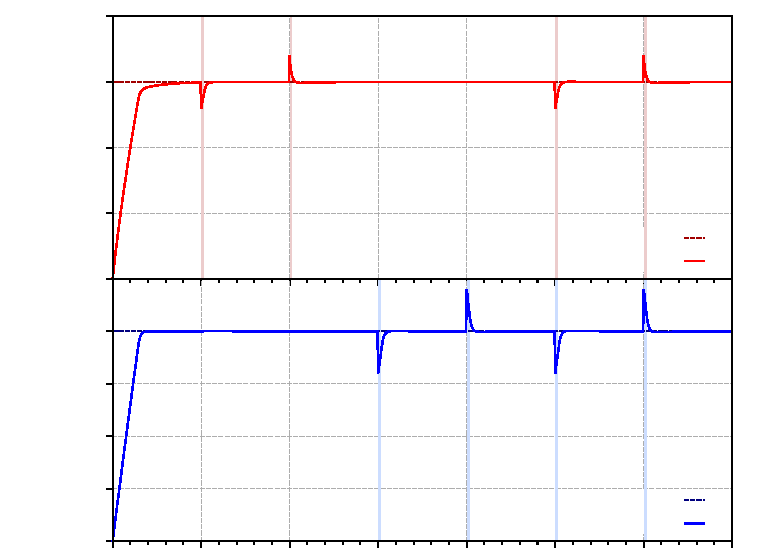
\includegraphics{fsedo}}%
    \gplfronttext
  \end{picture}%
\endgroup
}
        \vspace{0.5cm}
        \caption{UOSeF}
        \label{fig:fsedo}
    \end{minipage}
\end{figure}

\begin{figure}[htb]
    \begin{minipage}[b]{0.48\linewidth}
        \scalebox{0.65}{% GNUPLOT: LaTeX picture with Postscript
\begingroup
  \makeatletter
  \providecommand\color[2][]{%
    \GenericError{(gnuplot) \space\space\space\@spaces}{%
      Package color not loaded in conjunction with
      terminal option `colourtext'%
    }{See the gnuplot documentation for explanation.%
    }{Either use 'blacktext' in gnuplot or load the package
      color.sty in LaTeX.}%
    \renewcommand\color[2][]{}%
  }%
  \providecommand\includegraphics[2][]{%
    \GenericError{(gnuplot) \space\space\space\@spaces}{%
      Package graphicx or graphics not loaded%
    }{See the gnuplot documentation for explanation.%
    }{The gnuplot epslatex terminal needs graphicx.sty or graphics.sty.}%
    \renewcommand\includegraphics[2][]{}%
  }%
  \providecommand\rotatebox[2]{#2}%
  \@ifundefined{ifGPcolor}{%
    \newif\ifGPcolor
    \GPcolortrue
  }{}%
  \@ifundefined{ifGPblacktext}{%
    \newif\ifGPblacktext
    \GPblacktexttrue
  }{}%
  % define a \g@addto@macro without @ in the name:
  \let\gplgaddtomacro\g@addto@macro
  % define empty templates for all commands taking text:
  \gdef\gplbacktext{}%
  \gdef\gplfronttext{}%
  \makeatother
  \ifGPblacktext
    % no textcolor at all
    \def\colorrgb#1{}%
    \def\colorgray#1{}%
  \else
    % gray or color?
    \ifGPcolor
      \def\colorrgb#1{\color[rgb]{#1}}%
      \def\colorgray#1{\color[gray]{#1}}%
      \expandafter\def\csname LTw\endcsname{\color{white}}%
      \expandafter\def\csname LTb\endcsname{\color{black}}%
      \expandafter\def\csname LTa\endcsname{\color{black}}%
      \expandafter\def\csname LT0\endcsname{\color[rgb]{1,0,0}}%
      \expandafter\def\csname LT1\endcsname{\color[rgb]{0,1,0}}%
      \expandafter\def\csname LT2\endcsname{\color[rgb]{0,0,1}}%
      \expandafter\def\csname LT3\endcsname{\color[rgb]{1,0,1}}%
      \expandafter\def\csname LT4\endcsname{\color[rgb]{0,1,1}}%
      \expandafter\def\csname LT5\endcsname{\color[rgb]{1,1,0}}%
      \expandafter\def\csname LT6\endcsname{\color[rgb]{0,0,0}}%
      \expandafter\def\csname LT7\endcsname{\color[rgb]{1,0.3,0}}%
      \expandafter\def\csname LT8\endcsname{\color[rgb]{0.5,0.5,0.5}}%
    \else
      % gray
      \def\colorrgb#1{\color{black}}%
      \def\colorgray#1{\color[gray]{#1}}%
      \expandafter\def\csname LTw\endcsname{\color{white}}%
      \expandafter\def\csname LTb\endcsname{\color{black}}%
      \expandafter\def\csname LTa\endcsname{\color{black}}%
      \expandafter\def\csname LT0\endcsname{\color{black}}%
      \expandafter\def\csname LT1\endcsname{\color{black}}%
      \expandafter\def\csname LT2\endcsname{\color{black}}%
      \expandafter\def\csname LT3\endcsname{\color{black}}%
      \expandafter\def\csname LT4\endcsname{\color{black}}%
      \expandafter\def\csname LT5\endcsname{\color{black}}%
      \expandafter\def\csname LT6\endcsname{\color{black}}%
      \expandafter\def\csname LT7\endcsname{\color{black}}%
      \expandafter\def\csname LT8\endcsname{\color{black}}%
    \fi
  \fi
  \setlength{\unitlength}{0.0500bp}%
  \begin{picture}(7200.00,5040.00)%
    \gplgaddtomacro\gplbacktext{%
      \csname LTb\endcsname%
      \put(726,3150){\makebox(0,0)[r]{\strut{} 5}}%
      \csname LTb\endcsname%
      \put(726,3780){\makebox(0,0)[r]{\strut{} 10}}%
      \csname LTb\endcsname%
      \put(726,4409){\makebox(0,0)[r]{\strut{} 15}}%
      \csname LTb\endcsname%
      \put(726,5039){\makebox(0,0)[r]{\strut{} 20}}%
      \csname LTb\endcsname%
      \put(921,2237){\makebox(0,0){\strut{}}}%
      \csname LTb\endcsname%
      \put(1771,2237){\makebox(0,0){\strut{}}}%
      \csname LTb\endcsname%
      \put(2620,2237){\makebox(0,0){\strut{}}}%
      \csname LTb\endcsname%
      \put(3470,2237){\makebox(0,0){\strut{}}}%
      \csname LTb\endcsname%
      \put(4320,2237){\makebox(0,0){\strut{}}}%
      \csname LTb\endcsname%
      \put(5170,2237){\makebox(0,0){\strut{}}}%
      \csname LTb\endcsname%
      \put(6019,2237){\makebox(0,0){\strut{}}}%
      \csname LTb\endcsname%
      \put(6869,2237){\makebox(0,0){\strut{}}}%
      \put(352,3779){\rotatebox{-270}{\makebox(0,0){\strut{}Nível [cm]}}}%
    }%
    \gplgaddtomacro\gplfronttext{%
      \csname LTb\endcsname%
      \put(6278,2913){\makebox(0,0)[r]{\strut{}Ref. $T_1$}}%
      \csname LTb\endcsname%
      \put(6278,2693){\makebox(0,0)[r]{\strut{}Saída $T_1$}}%
    }%
    \gplgaddtomacro\gplbacktext{%
      \csname LTb\endcsname%
      \put(726,0){\makebox(0,0)[r]{\strut{} 0}}%
      \csname LTb\endcsname%
      \put(726,840){\makebox(0,0)[r]{\strut{} 10}}%
      \csname LTb\endcsname%
      \put(726,1680){\makebox(0,0)[r]{\strut{} 20}}%
      \csname LTb\endcsname%
      \put(726,2520){\makebox(0,0)[r]{\strut{} 30}}%
      \csname LTb\endcsname%
      \put(921,-283){\makebox(0,0){\strut{}0}}%
      \csname LTb\endcsname%
      \put(1771,-283){\makebox(0,0){\strut{}15}}%
      \csname LTb\endcsname%
      \put(2620,-283){\makebox(0,0){\strut{}30}}%
      \csname LTb\endcsname%
      \put(3470,-283){\makebox(0,0){\strut{}45}}%
      \csname LTb\endcsname%
      \put(4320,-283){\makebox(0,0){\strut{}60}}%
      \csname LTb\endcsname%
      \put(5170,-283){\makebox(0,0){\strut{}75}}%
      \csname LTb\endcsname%
      \put(6019,-283){\makebox(0,0){\strut{}90}}%
      \csname LTb\endcsname%
      \put(6869,-283){\makebox(0,0){\strut{}105}}%
      \put(352,1260){\rotatebox{-270}{\makebox(0,0){\strut{}Nível [cm]}}}%
      \put(3895,-613){\makebox(0,0){\strut{}Tempo [s]}}%
    }%
    \gplgaddtomacro\gplfronttext{%
      \csname LTb\endcsname%
      \put(6278,393){\makebox(0,0)[r]{\strut{}Ref. $T_2$}}%
      \csname LTb\endcsname%
      \put(6278,173){\makebox(0,0)[r]{\strut{}Saída $T_2$}}%
    }%
    \gplbacktext
    \put(0,0){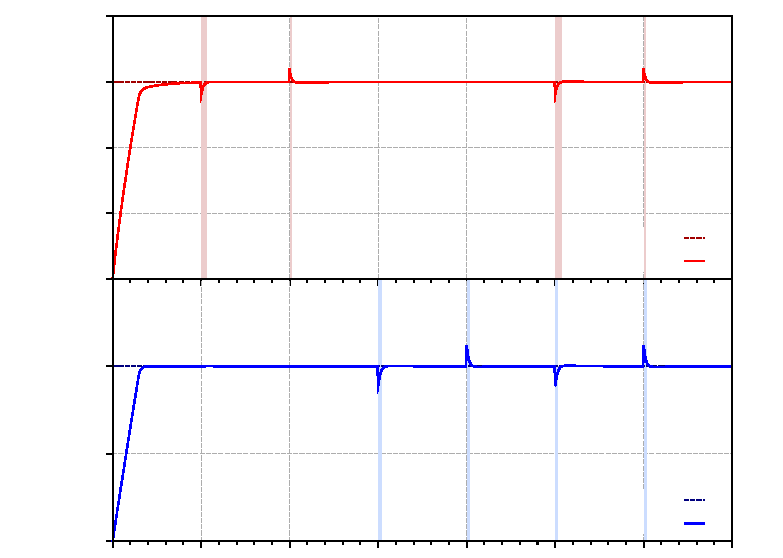
\includegraphics{fsivzt}}%
    \gplfronttext
  \end{picture}%
\endgroup
}
        \vspace{0.5cm}
        \caption{TLStF}
        \label{fig:fsivzt}
    \end{minipage}
    \hfill
    \begin{minipage}[b]{0.48\linewidth}
        \scalebox{0.65}{% GNUPLOT: LaTeX picture with Postscript
\begingroup
  \makeatletter
  \providecommand\color[2][]{%
    \GenericError{(gnuplot) \space\space\space\@spaces}{%
      Package color not loaded in conjunction with
      terminal option `colourtext'%
    }{See the gnuplot documentation for explanation.%
    }{Either use 'blacktext' in gnuplot or load the package
      color.sty in LaTeX.}%
    \renewcommand\color[2][]{}%
  }%
  \providecommand\includegraphics[2][]{%
    \GenericError{(gnuplot) \space\space\space\@spaces}{%
      Package graphicx or graphics not loaded%
    }{See the gnuplot documentation for explanation.%
    }{The gnuplot epslatex terminal needs graphicx.sty or graphics.sty.}%
    \renewcommand\includegraphics[2][]{}%
  }%
  \providecommand\rotatebox[2]{#2}%
  \@ifundefined{ifGPcolor}{%
    \newif\ifGPcolor
    \GPcolortrue
  }{}%
  \@ifundefined{ifGPblacktext}{%
    \newif\ifGPblacktext
    \GPblacktexttrue
  }{}%
  % define a \g@addto@macro without @ in the name:
  \let\gplgaddtomacro\g@addto@macro
  % define empty templates for all commands taking text:
  \gdef\gplbacktext{}%
  \gdef\gplfronttext{}%
  \makeatother
  \ifGPblacktext
    % no textcolor at all
    \def\colorrgb#1{}%
    \def\colorgray#1{}%
  \else
    % gray or color?
    \ifGPcolor
      \def\colorrgb#1{\color[rgb]{#1}}%
      \def\colorgray#1{\color[gray]{#1}}%
      \expandafter\def\csname LTw\endcsname{\color{white}}%
      \expandafter\def\csname LTb\endcsname{\color{black}}%
      \expandafter\def\csname LTa\endcsname{\color{black}}%
      \expandafter\def\csname LT0\endcsname{\color[rgb]{1,0,0}}%
      \expandafter\def\csname LT1\endcsname{\color[rgb]{0,1,0}}%
      \expandafter\def\csname LT2\endcsname{\color[rgb]{0,0,1}}%
      \expandafter\def\csname LT3\endcsname{\color[rgb]{1,0,1}}%
      \expandafter\def\csname LT4\endcsname{\color[rgb]{0,1,1}}%
      \expandafter\def\csname LT5\endcsname{\color[rgb]{1,1,0}}%
      \expandafter\def\csname LT6\endcsname{\color[rgb]{0,0,0}}%
      \expandafter\def\csname LT7\endcsname{\color[rgb]{1,0.3,0}}%
      \expandafter\def\csname LT8\endcsname{\color[rgb]{0.5,0.5,0.5}}%
    \else
      % gray
      \def\colorrgb#1{\color{black}}%
      \def\colorgray#1{\color[gray]{#1}}%
      \expandafter\def\csname LTw\endcsname{\color{white}}%
      \expandafter\def\csname LTb\endcsname{\color{black}}%
      \expandafter\def\csname LTa\endcsname{\color{black}}%
      \expandafter\def\csname LT0\endcsname{\color{black}}%
      \expandafter\def\csname LT1\endcsname{\color{black}}%
      \expandafter\def\csname LT2\endcsname{\color{black}}%
      \expandafter\def\csname LT3\endcsname{\color{black}}%
      \expandafter\def\csname LT4\endcsname{\color{black}}%
      \expandafter\def\csname LT5\endcsname{\color{black}}%
      \expandafter\def\csname LT6\endcsname{\color{black}}%
      \expandafter\def\csname LT7\endcsname{\color{black}}%
      \expandafter\def\csname LT8\endcsname{\color{black}}%
    \fi
  \fi
  \setlength{\unitlength}{0.0500bp}%
  \begin{picture}(7200.00,5040.00)%
    \gplgaddtomacro\gplbacktext{%
      \csname LTb\endcsname%
      \put(726,3150){\makebox(0,0)[r]{\strut{} 5}}%
      \csname LTb\endcsname%
      \put(726,3780){\makebox(0,0)[r]{\strut{} 10}}%
      \csname LTb\endcsname%
      \put(726,4409){\makebox(0,0)[r]{\strut{} 15}}%
      \csname LTb\endcsname%
      \put(726,5039){\makebox(0,0)[r]{\strut{} 20}}%
      \csname LTb\endcsname%
      \put(921,2237){\makebox(0,0){\strut{}}}%
      \csname LTb\endcsname%
      \put(1771,2237){\makebox(0,0){\strut{}}}%
      \csname LTb\endcsname%
      \put(2620,2237){\makebox(0,0){\strut{}}}%
      \csname LTb\endcsname%
      \put(3470,2237){\makebox(0,0){\strut{}}}%
      \csname LTb\endcsname%
      \put(4320,2237){\makebox(0,0){\strut{}}}%
      \csname LTb\endcsname%
      \put(5170,2237){\makebox(0,0){\strut{}}}%
      \csname LTb\endcsname%
      \put(6019,2237){\makebox(0,0){\strut{}}}%
      \csname LTb\endcsname%
      \put(6869,2237){\makebox(0,0){\strut{}}}%
      \put(352,3779){\rotatebox{-270}{\makebox(0,0){\strut{}Nível [cm]}}}%
    }%
    \gplgaddtomacro\gplfronttext{%
      \csname LTb\endcsname%
      \put(6278,2913){\makebox(0,0)[r]{\strut{}Ref. $T_1$}}%
      \csname LTb\endcsname%
      \put(6278,2693){\makebox(0,0)[r]{\strut{}Saída $T_1$}}%
    }%
    \gplgaddtomacro\gplbacktext{%
      \csname LTb\endcsname%
      \put(726,0){\makebox(0,0)[r]{\strut{} 0}}%
      \csname LTb\endcsname%
      \put(726,504){\makebox(0,0)[r]{\strut{} 5}}%
      \csname LTb\endcsname%
      \put(726,1008){\makebox(0,0)[r]{\strut{} 10}}%
      \csname LTb\endcsname%
      \put(726,1512){\makebox(0,0)[r]{\strut{} 15}}%
      \csname LTb\endcsname%
      \put(726,2016){\makebox(0,0)[r]{\strut{} 20}}%
      \csname LTb\endcsname%
      \put(726,2520){\makebox(0,0)[r]{\strut{} 25}}%
      \csname LTb\endcsname%
      \put(921,-283){\makebox(0,0){\strut{}0}}%
      \csname LTb\endcsname%
      \put(1771,-283){\makebox(0,0){\strut{}15}}%
      \csname LTb\endcsname%
      \put(2620,-283){\makebox(0,0){\strut{}30}}%
      \csname LTb\endcsname%
      \put(3470,-283){\makebox(0,0){\strut{}45}}%
      \csname LTb\endcsname%
      \put(4320,-283){\makebox(0,0){\strut{}60}}%
      \csname LTb\endcsname%
      \put(5170,-283){\makebox(0,0){\strut{}75}}%
      \csname LTb\endcsname%
      \put(6019,-283){\makebox(0,0){\strut{}90}}%
      \csname LTb\endcsname%
      \put(6869,-283){\makebox(0,0){\strut{}105}}%
      \put(352,1260){\rotatebox{-270}{\makebox(0,0){\strut{}Nível [cm]}}}%
      \put(3895,-613){\makebox(0,0){\strut{}Tempo [s]}}%
    }%
    \gplgaddtomacro\gplfronttext{%
      \csname LTb\endcsname%
      \put(6278,393){\makebox(0,0)[r]{\strut{}Ref. $T_2$}}%
      \csname LTb\endcsname%
      \put(6278,173){\makebox(0,0)[r]{\strut{}Saída $T_2$}}%
    }%
    \gplbacktext
    \put(0,0){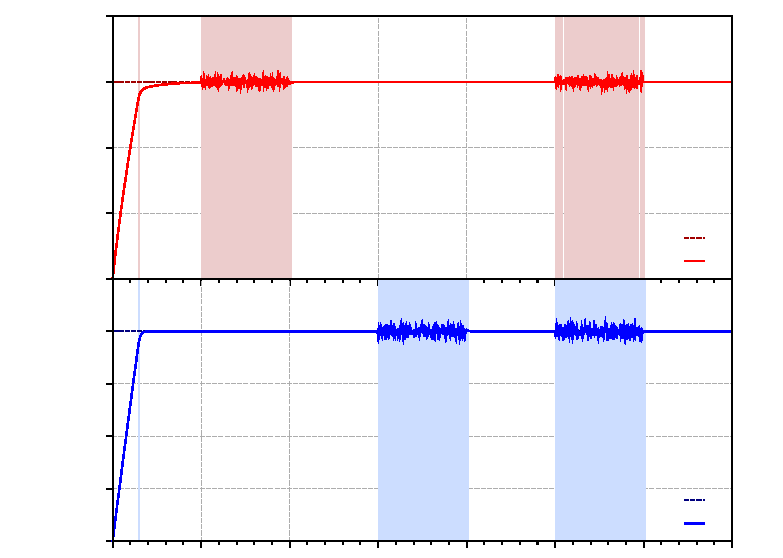
\includegraphics{fsesr}}%
    \gplfronttext
  \end{picture}%
\endgroup
}
        \vspace{0.5cm}
        \caption{NSSeF}
        \label{fig:fsesr}
    \end{minipage}
\end{figure}

Observa-se nessa figura que o sistema consegue identificar a presença da falha
assim que o valor do parâmetro é modificado. Após esse período, os controladores
conseguem ``compensar'' a falha, enviando mais tensão para a bomba e,
consequentemente, fazendo com que o nível retorne à referência. Observa-se,
entretanto, que essa ``compensação'' se dá de maneira inadequada, tendo em vista
que a leitura do nível estará com um erro de 20\%. 

Dessa forma, quando o valor lido pelos sensores for de 24\ cm, o tanque estará
prestes a transbordar, atingindo, na verdade, o limite superior de 30\ cm. Em
uma aplicação acadêmica tal situação pode não representar nenhum risco aos
equipamentos além daqueles em que a água venha a causar. Por outro lado, em
aplicações críticas essa ``compensação'' pode vir a causar diversos prejuízos.

O sistema se comportou de maneira semelhante à essa na UOSeF e na TLStF,
conforme observado nas Figs. \ref{fig:fsedo} e \ref{fig:fsivzt}. Essa semelhança
pode vir a dificultar a identificação dessas falhas quando as redes estiverem
agindo paralelamente.

Os resultados obtidos para essas falhas não estão condizentes com a Tab.
\ref{tab:best_ann}. Tal situação pode estar acontecendo porque as redes
identificaram uma dinâmica para variações rápidas através de sinais de excitação
pseudo aleatórios, não conseguindo identificar variações bruscas e continuadas.

Assim, uma possível alternativa para contornar esse problema, seria a de se
utilizar flags binárias, ativadas no momento em que fosse detectada a primeira
variação e desativadas na detecção seguinte. Essas flags indicariam para o
sistema que a falha está agindo durante todo o intervalo de tempo em que
estivessem ativas.

Uma outra simulação mostrou que a NSSeF foi facilmente identificada pelo
sistema, como pode ser visto na Fig. \ref{fig:fsesr}. Observa-se entretanto que,
por se tratar de um ruído com distribuição uniforme ($\pm 2\%$), o sistema não
consegue identificar a falha em alguns pontos. Nesses pontos, pode-se perceber
que o valor gerado pela função {\tt rand} mantém o sinal próximo à referência.

\begin{figure}[htb]
    \begin{minipage}[b]{0.48\linewidth}
        \scalebox{0.65}{% GNUPLOT: LaTeX picture with Postscript
\begingroup
  \makeatletter
  \providecommand\color[2][]{%
    \GenericError{(gnuplot) \space\space\space\@spaces}{%
      Package color not loaded in conjunction with
      terminal option `colourtext'%
    }{See the gnuplot documentation for explanation.%
    }{Either use 'blacktext' in gnuplot or load the package
      color.sty in LaTeX.}%
    \renewcommand\color[2][]{}%
  }%
  \providecommand\includegraphics[2][]{%
    \GenericError{(gnuplot) \space\space\space\@spaces}{%
      Package graphicx or graphics not loaded%
    }{See the gnuplot documentation for explanation.%
    }{The gnuplot epslatex terminal needs graphicx.sty or graphics.sty.}%
    \renewcommand\includegraphics[2][]{}%
  }%
  \providecommand\rotatebox[2]{#2}%
  \@ifundefined{ifGPcolor}{%
    \newif\ifGPcolor
    \GPcolortrue
  }{}%
  \@ifundefined{ifGPblacktext}{%
    \newif\ifGPblacktext
    \GPblacktexttrue
  }{}%
  % define a \g@addto@macro without @ in the name:
  \let\gplgaddtomacro\g@addto@macro
  % define empty templates for all commands taking text:
  \gdef\gplbacktext{}%
  \gdef\gplfronttext{}%
  \makeatother
  \ifGPblacktext
    % no textcolor at all
    \def\colorrgb#1{}%
    \def\colorgray#1{}%
  \else
    % gray or color?
    \ifGPcolor
      \def\colorrgb#1{\color[rgb]{#1}}%
      \def\colorgray#1{\color[gray]{#1}}%
      \expandafter\def\csname LTw\endcsname{\color{white}}%
      \expandafter\def\csname LTb\endcsname{\color{black}}%
      \expandafter\def\csname LTa\endcsname{\color{black}}%
      \expandafter\def\csname LT0\endcsname{\color[rgb]{1,0,0}}%
      \expandafter\def\csname LT1\endcsname{\color[rgb]{0,1,0}}%
      \expandafter\def\csname LT2\endcsname{\color[rgb]{0,0,1}}%
      \expandafter\def\csname LT3\endcsname{\color[rgb]{1,0,1}}%
      \expandafter\def\csname LT4\endcsname{\color[rgb]{0,1,1}}%
      \expandafter\def\csname LT5\endcsname{\color[rgb]{1,1,0}}%
      \expandafter\def\csname LT6\endcsname{\color[rgb]{0,0,0}}%
      \expandafter\def\csname LT7\endcsname{\color[rgb]{1,0.3,0}}%
      \expandafter\def\csname LT8\endcsname{\color[rgb]{0.5,0.5,0.5}}%
    \else
      % gray
      \def\colorrgb#1{\color{black}}%
      \def\colorgray#1{\color[gray]{#1}}%
      \expandafter\def\csname LTw\endcsname{\color{white}}%
      \expandafter\def\csname LTb\endcsname{\color{black}}%
      \expandafter\def\csname LTa\endcsname{\color{black}}%
      \expandafter\def\csname LT0\endcsname{\color{black}}%
      \expandafter\def\csname LT1\endcsname{\color{black}}%
      \expandafter\def\csname LT2\endcsname{\color{black}}%
      \expandafter\def\csname LT3\endcsname{\color{black}}%
      \expandafter\def\csname LT4\endcsname{\color{black}}%
      \expandafter\def\csname LT5\endcsname{\color{black}}%
      \expandafter\def\csname LT6\endcsname{\color{black}}%
      \expandafter\def\csname LT7\endcsname{\color{black}}%
      \expandafter\def\csname LT8\endcsname{\color{black}}%
    \fi
  \fi
  \setlength{\unitlength}{0.0500bp}%
  \begin{picture}(7200.00,5040.00)%
    \gplgaddtomacro\gplbacktext{%
      \csname LTb\endcsname%
      \put(726,3150){\makebox(0,0)[r]{\strut{} 5}}%
      \csname LTb\endcsname%
      \put(726,3780){\makebox(0,0)[r]{\strut{} 10}}%
      \csname LTb\endcsname%
      \put(726,4409){\makebox(0,0)[r]{\strut{} 15}}%
      \csname LTb\endcsname%
      \put(726,5039){\makebox(0,0)[r]{\strut{} 20}}%
      \csname LTb\endcsname%
      \put(921,2237){\makebox(0,0){\strut{}}}%
      \csname LTb\endcsname%
      \put(1771,2237){\makebox(0,0){\strut{}}}%
      \csname LTb\endcsname%
      \put(2620,2237){\makebox(0,0){\strut{}}}%
      \csname LTb\endcsname%
      \put(3470,2237){\makebox(0,0){\strut{}}}%
      \csname LTb\endcsname%
      \put(4320,2237){\makebox(0,0){\strut{}}}%
      \csname LTb\endcsname%
      \put(5170,2237){\makebox(0,0){\strut{}}}%
      \csname LTb\endcsname%
      \put(6019,2237){\makebox(0,0){\strut{}}}%
      \csname LTb\endcsname%
      \put(6869,2237){\makebox(0,0){\strut{}}}%
      \put(352,3779){\rotatebox{-270}{\makebox(0,0){\strut{}Level [cm]}}}%
    }%
    \gplgaddtomacro\gplfronttext{%
      \csname LTb\endcsname%
      \put(6278,2913){\makebox(0,0)[r]{\strut{}Setpoint $T_1$}}%
      \csname LTb\endcsname%
      \put(6278,2693){\makebox(0,0)[r]{\strut{}Output $T_1$}}%
    }%
    \gplgaddtomacro\gplbacktext{%
      \csname LTb\endcsname%
      \put(726,0){\makebox(0,0)[r]{\strut{} 0}}%
      \csname LTb\endcsname%
      \put(726,840){\makebox(0,0)[r]{\strut{} 10}}%
      \csname LTb\endcsname%
      \put(726,1680){\makebox(0,0)[r]{\strut{} 20}}%
      \csname LTb\endcsname%
      \put(726,2520){\makebox(0,0)[r]{\strut{} 30}}%
      \csname LTb\endcsname%
      \put(921,-283){\makebox(0,0){\strut{}0}}%
      \csname LTb\endcsname%
      \put(1771,-283){\makebox(0,0){\strut{}15}}%
      \csname LTb\endcsname%
      \put(2620,-283){\makebox(0,0){\strut{}30}}%
      \csname LTb\endcsname%
      \put(3470,-283){\makebox(0,0){\strut{}45}}%
      \csname LTb\endcsname%
      \put(4320,-283){\makebox(0,0){\strut{}60}}%
      \csname LTb\endcsname%
      \put(5170,-283){\makebox(0,0){\strut{}75}}%
      \csname LTb\endcsname%
      \put(6019,-283){\makebox(0,0){\strut{}90}}%
      \csname LTb\endcsname%
      \put(6869,-283){\makebox(0,0){\strut{}105}}%
      \put(352,1260){\rotatebox{-270}{\makebox(0,0){\strut{}Level [cm]}}}%
      \put(3895,-613){\makebox(0,0){\strut{}Time [s]}}%
    }%
    \gplgaddtomacro\gplfronttext{%
      \csname LTb\endcsname%
      \put(6278,393){\makebox(0,0)[r]{\strut{}Setpoint $T_2$}}%
      \csname LTb\endcsname%
      \put(6278,173){\makebox(0,0)[r]{\strut{}Output $T_2$}}%
    }%
    \gplbacktext
    \put(0,0){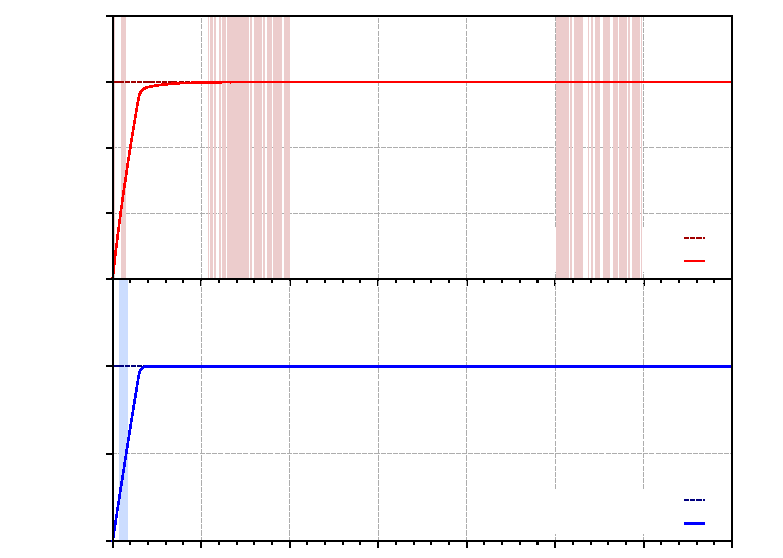
\includegraphics{fasr}}%
    \gplfronttext
  \end{picture}%
\endgroup
}
        \vspace{0.5cm}
        \caption{NSAF}
        \label{fig:fasr}
    \end{minipage}
    \hfill
    \begin{minipage}[b]{0.48\linewidth}
        \scalebox{0.65}{% GNUPLOT: LaTeX picture with Postscript
\begingroup
  \makeatletter
  \providecommand\color[2][]{%
    \GenericError{(gnuplot) \space\space\space\@spaces}{%
      Package color not loaded in conjunction with
      terminal option `colourtext'%
    }{See the gnuplot documentation for explanation.%
    }{Either use 'blacktext' in gnuplot or load the package
      color.sty in LaTeX.}%
    \renewcommand\color[2][]{}%
  }%
  \providecommand\includegraphics[2][]{%
    \GenericError{(gnuplot) \space\space\space\@spaces}{%
      Package graphicx or graphics not loaded%
    }{See the gnuplot documentation for explanation.%
    }{The gnuplot epslatex terminal needs graphicx.sty or graphics.sty.}%
    \renewcommand\includegraphics[2][]{}%
  }%
  \providecommand\rotatebox[2]{#2}%
  \@ifundefined{ifGPcolor}{%
    \newif\ifGPcolor
    \GPcolortrue
  }{}%
  \@ifundefined{ifGPblacktext}{%
    \newif\ifGPblacktext
    \GPblacktexttrue
  }{}%
  % define a \g@addto@macro without @ in the name:
  \let\gplgaddtomacro\g@addto@macro
  % define empty templates for all commands taking text:
  \gdef\gplbacktext{}%
  \gdef\gplfronttext{}%
  \makeatother
  \ifGPblacktext
    % no textcolor at all
    \def\colorrgb#1{}%
    \def\colorgray#1{}%
  \else
    % gray or color?
    \ifGPcolor
      \def\colorrgb#1{\color[rgb]{#1}}%
      \def\colorgray#1{\color[gray]{#1}}%
      \expandafter\def\csname LTw\endcsname{\color{white}}%
      \expandafter\def\csname LTb\endcsname{\color{black}}%
      \expandafter\def\csname LTa\endcsname{\color{black}}%
      \expandafter\def\csname LT0\endcsname{\color[rgb]{1,0,0}}%
      \expandafter\def\csname LT1\endcsname{\color[rgb]{0,1,0}}%
      \expandafter\def\csname LT2\endcsname{\color[rgb]{0,0,1}}%
      \expandafter\def\csname LT3\endcsname{\color[rgb]{1,0,1}}%
      \expandafter\def\csname LT4\endcsname{\color[rgb]{0,1,1}}%
      \expandafter\def\csname LT5\endcsname{\color[rgb]{1,1,0}}%
      \expandafter\def\csname LT6\endcsname{\color[rgb]{0,0,0}}%
      \expandafter\def\csname LT7\endcsname{\color[rgb]{1,0.3,0}}%
      \expandafter\def\csname LT8\endcsname{\color[rgb]{0.5,0.5,0.5}}%
    \else
      % gray
      \def\colorrgb#1{\color{black}}%
      \def\colorgray#1{\color[gray]{#1}}%
      \expandafter\def\csname LTw\endcsname{\color{white}}%
      \expandafter\def\csname LTb\endcsname{\color{black}}%
      \expandafter\def\csname LTa\endcsname{\color{black}}%
      \expandafter\def\csname LT0\endcsname{\color{black}}%
      \expandafter\def\csname LT1\endcsname{\color{black}}%
      \expandafter\def\csname LT2\endcsname{\color{black}}%
      \expandafter\def\csname LT3\endcsname{\color{black}}%
      \expandafter\def\csname LT4\endcsname{\color{black}}%
      \expandafter\def\csname LT5\endcsname{\color{black}}%
      \expandafter\def\csname LT6\endcsname{\color{black}}%
      \expandafter\def\csname LT7\endcsname{\color{black}}%
      \expandafter\def\csname LT8\endcsname{\color{black}}%
    \fi
  \fi
  \setlength{\unitlength}{0.0500bp}%
  \begin{picture}(7200.00,5040.00)%
    \gplgaddtomacro\gplbacktext{%
      \csname LTb\endcsname%
      \put(726,2800){\makebox(0,0)[r]{\strut{} 5}}%
      \csname LTb\endcsname%
      \put(726,3080){\makebox(0,0)[r]{\strut{} 10}}%
      \csname LTb\endcsname%
      \put(726,3360){\makebox(0,0)[r]{\strut{} 15}}%
      \csname LTb\endcsname%
      \put(726,3640){\makebox(0,0)[r]{\strut{} 20}}%
      \csname LTb\endcsname%
      \put(726,3919){\makebox(0,0)[r]{\strut{} 25}}%
      \csname LTb\endcsname%
      \put(726,4199){\makebox(0,0)[r]{\strut{} 30}}%
      \csname LTb\endcsname%
      \put(726,4479){\makebox(0,0)[r]{\strut{} 35}}%
      \csname LTb\endcsname%
      \put(726,4759){\makebox(0,0)[r]{\strut{} 40}}%
      \csname LTb\endcsname%
      \put(726,5039){\makebox(0,0)[r]{\strut{} 45}}%
      \csname LTb\endcsname%
      \put(921,2237){\makebox(0,0){\strut{}}}%
      \csname LTb\endcsname%
      \put(1771,2237){\makebox(0,0){\strut{}}}%
      \csname LTb\endcsname%
      \put(2620,2237){\makebox(0,0){\strut{}}}%
      \csname LTb\endcsname%
      \put(3470,2237){\makebox(0,0){\strut{}}}%
      \csname LTb\endcsname%
      \put(4320,2237){\makebox(0,0){\strut{}}}%
      \csname LTb\endcsname%
      \put(5170,2237){\makebox(0,0){\strut{}}}%
      \csname LTb\endcsname%
      \put(6019,2237){\makebox(0,0){\strut{}}}%
      \csname LTb\endcsname%
      \put(6869,2237){\makebox(0,0){\strut{}}}%
      \put(352,3779){\rotatebox{-270}{\makebox(0,0){\strut{}Level [cm]}}}%
    }%
    \gplgaddtomacro\gplfronttext{%
      \csname LTb\endcsname%
      \put(6278,2913){\makebox(0,0)[r]{\strut{}Setpoint $T_1$}}%
      \csname LTb\endcsname%
      \put(6278,2693){\makebox(0,0)[r]{\strut{}Output $T_1$}}%
    }%
    \gplgaddtomacro\gplbacktext{%
      \csname LTb\endcsname%
      \put(726,0){\makebox(0,0)[r]{\strut{} 0}}%
      \csname LTb\endcsname%
      \put(726,315){\makebox(0,0)[r]{\strut{} 10}}%
      \csname LTb\endcsname%
      \put(726,630){\makebox(0,0)[r]{\strut{} 20}}%
      \csname LTb\endcsname%
      \put(726,945){\makebox(0,0)[r]{\strut{} 30}}%
      \csname LTb\endcsname%
      \put(726,1260){\makebox(0,0)[r]{\strut{} 40}}%
      \csname LTb\endcsname%
      \put(726,1575){\makebox(0,0)[r]{\strut{} 50}}%
      \csname LTb\endcsname%
      \put(726,1890){\makebox(0,0)[r]{\strut{} 60}}%
      \csname LTb\endcsname%
      \put(726,2205){\makebox(0,0)[r]{\strut{} 70}}%
      \csname LTb\endcsname%
      \put(726,2520){\makebox(0,0)[r]{\strut{} 80}}%
      \csname LTb\endcsname%
      \put(921,-283){\makebox(0,0){\strut{}0}}%
      \csname LTb\endcsname%
      \put(1771,-283){\makebox(0,0){\strut{}15}}%
      \csname LTb\endcsname%
      \put(2620,-283){\makebox(0,0){\strut{}30}}%
      \csname LTb\endcsname%
      \put(3470,-283){\makebox(0,0){\strut{}45}}%
      \csname LTb\endcsname%
      \put(4320,-283){\makebox(0,0){\strut{}60}}%
      \csname LTb\endcsname%
      \put(5170,-283){\makebox(0,0){\strut{}75}}%
      \csname LTb\endcsname%
      \put(6019,-283){\makebox(0,0){\strut{}90}}%
      \csname LTb\endcsname%
      \put(6869,-283){\makebox(0,0){\strut{}105}}%
      \put(352,1260){\rotatebox{-270}{\makebox(0,0){\strut{}Level [cm]}}}%
      \put(3895,-613){\makebox(0,0){\strut{}Time [s]}}%
    }%
    \gplgaddtomacro\gplfronttext{%
      \csname LTb\endcsname%
      \put(6278,393){\makebox(0,0)[r]{\strut{}Setpoint $T_2$}}%
      \csname LTb\endcsname%
      \put(6278,173){\makebox(0,0)[r]{\strut{}Output $T_2$}}%
    }%
    \gplbacktext
    \put(0,0){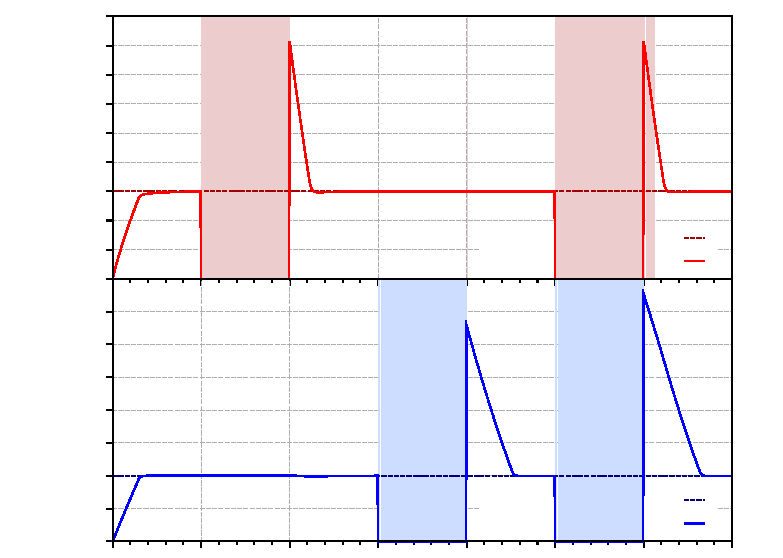
\includegraphics{fseq}}%
    \gplfronttext
  \end{picture}%
\endgroup
}
        \vspace{0.5cm}
        \caption{BSeF}
        \label{fig:fseq}
    \end{minipage}
\end{figure}

Ao contrário da NSSeF, a simulação realizada para a NSAF não foi tão facilmente
identificada, como pode ser visto na Fig. \ref{fig:fasr}. Os resultados obtidos
para $T_1$ podem até ser considerados razoáveis, enquanto que os resultados para
$T_2$ são visivelmente inaceitáveis, tendo em vista que nenhum dos pontos em que
a falha deveria ter sido identificada foram reconhecidos pela rede. Apesar
disso, observa-se que os resultados estão condizentes com a Tab.
\ref{tab:melhores_redes_detec}, em que o total de erros de detecção supera 40\%.

Todas as demais falhas restantes também foram facilmente identificadas pelo
sistema, como pode ser observado nas Figs. \ref{fig:fseq} a \ref{fig:fsieos}. 

\begin{figure}[htb]
    \begin{minipage}[b]{0.48\linewidth}
        \scalebox{0.65}{% GNUPLOT: LaTeX picture with Postscript
\begingroup
  \makeatletter
  \providecommand\color[2][]{%
    \GenericError{(gnuplot) \space\space\space\@spaces}{%
      Package color not loaded in conjunction with
      terminal option `colourtext'%
    }{See the gnuplot documentation for explanation.%
    }{Either use 'blacktext' in gnuplot or load the package
      color.sty in LaTeX.}%
    \renewcommand\color[2][]{}%
  }%
  \providecommand\includegraphics[2][]{%
    \GenericError{(gnuplot) \space\space\space\@spaces}{%
      Package graphicx or graphics not loaded%
    }{See the gnuplot documentation for explanation.%
    }{The gnuplot epslatex terminal needs graphicx.sty or graphics.sty.}%
    \renewcommand\includegraphics[2][]{}%
  }%
  \providecommand\rotatebox[2]{#2}%
  \@ifundefined{ifGPcolor}{%
    \newif\ifGPcolor
    \GPcolortrue
  }{}%
  \@ifundefined{ifGPblacktext}{%
    \newif\ifGPblacktext
    \GPblacktexttrue
  }{}%
  % define a \g@addto@macro without @ in the name:
  \let\gplgaddtomacro\g@addto@macro
  % define empty templates for all commands taking text:
  \gdef\gplbacktext{}%
  \gdef\gplfronttext{}%
  \makeatother
  \ifGPblacktext
    % no textcolor at all
    \def\colorrgb#1{}%
    \def\colorgray#1{}%
  \else
    % gray or color?
    \ifGPcolor
      \def\colorrgb#1{\color[rgb]{#1}}%
      \def\colorgray#1{\color[gray]{#1}}%
      \expandafter\def\csname LTw\endcsname{\color{white}}%
      \expandafter\def\csname LTb\endcsname{\color{black}}%
      \expandafter\def\csname LTa\endcsname{\color{black}}%
      \expandafter\def\csname LT0\endcsname{\color[rgb]{1,0,0}}%
      \expandafter\def\csname LT1\endcsname{\color[rgb]{0,1,0}}%
      \expandafter\def\csname LT2\endcsname{\color[rgb]{0,0,1}}%
      \expandafter\def\csname LT3\endcsname{\color[rgb]{1,0,1}}%
      \expandafter\def\csname LT4\endcsname{\color[rgb]{0,1,1}}%
      \expandafter\def\csname LT5\endcsname{\color[rgb]{1,1,0}}%
      \expandafter\def\csname LT6\endcsname{\color[rgb]{0,0,0}}%
      \expandafter\def\csname LT7\endcsname{\color[rgb]{1,0.3,0}}%
      \expandafter\def\csname LT8\endcsname{\color[rgb]{0.5,0.5,0.5}}%
    \else
      % gray
      \def\colorrgb#1{\color{black}}%
      \def\colorgray#1{\color[gray]{#1}}%
      \expandafter\def\csname LTw\endcsname{\color{white}}%
      \expandafter\def\csname LTb\endcsname{\color{black}}%
      \expandafter\def\csname LTa\endcsname{\color{black}}%
      \expandafter\def\csname LT0\endcsname{\color{black}}%
      \expandafter\def\csname LT1\endcsname{\color{black}}%
      \expandafter\def\csname LT2\endcsname{\color{black}}%
      \expandafter\def\csname LT3\endcsname{\color{black}}%
      \expandafter\def\csname LT4\endcsname{\color{black}}%
      \expandafter\def\csname LT5\endcsname{\color{black}}%
      \expandafter\def\csname LT6\endcsname{\color{black}}%
      \expandafter\def\csname LT7\endcsname{\color{black}}%
      \expandafter\def\csname LT8\endcsname{\color{black}}%
    \fi
  \fi
  \setlength{\unitlength}{0.0500bp}%
  \begin{picture}(7200.00,5040.00)%
    \gplgaddtomacro\gplbacktext{%
      \csname LTb\endcsname%
      \put(726,3150){\makebox(0,0)[r]{\strut{} 5}}%
      \csname LTb\endcsname%
      \put(726,3780){\makebox(0,0)[r]{\strut{} 10}}%
      \csname LTb\endcsname%
      \put(726,4409){\makebox(0,0)[r]{\strut{} 15}}%
      \csname LTb\endcsname%
      \put(726,5039){\makebox(0,0)[r]{\strut{} 20}}%
      \csname LTb\endcsname%
      \put(921,2237){\makebox(0,0){\strut{}}}%
      \csname LTb\endcsname%
      \put(1771,2237){\makebox(0,0){\strut{}}}%
      \csname LTb\endcsname%
      \put(2620,2237){\makebox(0,0){\strut{}}}%
      \csname LTb\endcsname%
      \put(3470,2237){\makebox(0,0){\strut{}}}%
      \csname LTb\endcsname%
      \put(4320,2237){\makebox(0,0){\strut{}}}%
      \csname LTb\endcsname%
      \put(5170,2237){\makebox(0,0){\strut{}}}%
      \csname LTb\endcsname%
      \put(6019,2237){\makebox(0,0){\strut{}}}%
      \csname LTb\endcsname%
      \put(6869,2237){\makebox(0,0){\strut{}}}%
      \put(352,3779){\rotatebox{-270}{\makebox(0,0){\strut{}Nível [cm]}}}%
    }%
    \gplgaddtomacro\gplfronttext{%
      \csname LTb\endcsname%
      \put(6278,2913){\makebox(0,0)[r]{\strut{}Ref. $T_1$}}%
      \csname LTb\endcsname%
      \put(6278,2693){\makebox(0,0)[r]{\strut{}Saída $T_1$}}%
    }%
    \gplgaddtomacro\gplbacktext{%
      \csname LTb\endcsname%
      \put(726,0){\makebox(0,0)[r]{\strut{} 0}}%
      \csname LTb\endcsname%
      \put(726,840){\makebox(0,0)[r]{\strut{} 10}}%
      \csname LTb\endcsname%
      \put(726,1680){\makebox(0,0)[r]{\strut{} 20}}%
      \csname LTb\endcsname%
      \put(726,2520){\makebox(0,0)[r]{\strut{} 30}}%
      \csname LTb\endcsname%
      \put(921,-283){\makebox(0,0){\strut{}0}}%
      \csname LTb\endcsname%
      \put(1771,-283){\makebox(0,0){\strut{}15}}%
      \csname LTb\endcsname%
      \put(2620,-283){\makebox(0,0){\strut{}30}}%
      \csname LTb\endcsname%
      \put(3470,-283){\makebox(0,0){\strut{}45}}%
      \csname LTb\endcsname%
      \put(4320,-283){\makebox(0,0){\strut{}60}}%
      \csname LTb\endcsname%
      \put(5170,-283){\makebox(0,0){\strut{}75}}%
      \csname LTb\endcsname%
      \put(6019,-283){\makebox(0,0){\strut{}90}}%
      \csname LTb\endcsname%
      \put(6869,-283){\makebox(0,0){\strut{}105}}%
      \put(352,1260){\rotatebox{-270}{\makebox(0,0){\strut{}Nível [cm]}}}%
      \put(3895,-613){\makebox(0,0){\strut{}Tempo [s]}}%
    }%
    \gplgaddtomacro\gplfronttext{%
      \csname LTb\endcsname%
      \put(6278,393){\makebox(0,0)[r]{\strut{}Ref. $T_2$}}%
      \csname LTb\endcsname%
      \put(6278,173){\makebox(0,0)[r]{\strut{}Saída $T_2$}}%
    }%
    \gplbacktext
    \put(0,0){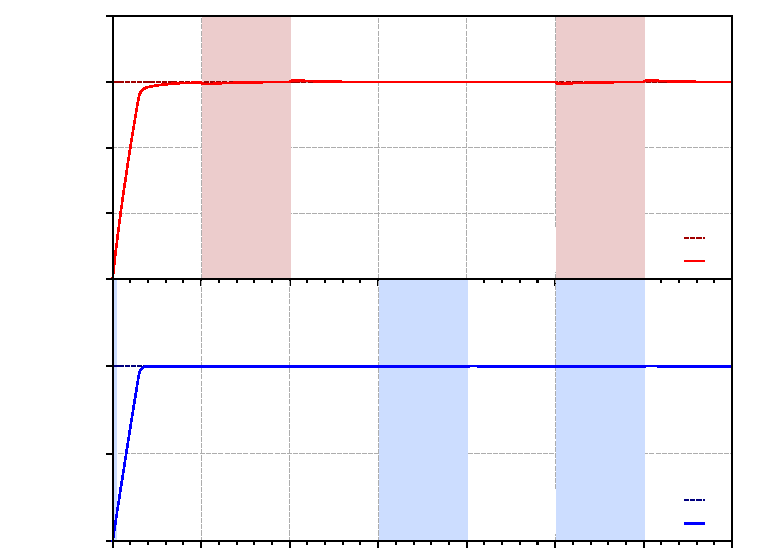
\includegraphics{fadg}}%
    \gplfronttext
  \end{picture}%
\endgroup
}
        \vspace{0.5cm}
        \caption{UGAF}
        \label{fig:fadg}
    \end{minipage}
    \hfill
    \begin{minipage}[b]{0.48\linewidth}
        \scalebox{0.65}{% GNUPLOT: LaTeX picture with Postscript
\begingroup
  \makeatletter
  \providecommand\color[2][]{%
    \GenericError{(gnuplot) \space\space\space\@spaces}{%
      Package color not loaded in conjunction with
      terminal option `colourtext'%
    }{See the gnuplot documentation for explanation.%
    }{Either use 'blacktext' in gnuplot or load the package
      color.sty in LaTeX.}%
    \renewcommand\color[2][]{}%
  }%
  \providecommand\includegraphics[2][]{%
    \GenericError{(gnuplot) \space\space\space\@spaces}{%
      Package graphicx or graphics not loaded%
    }{See the gnuplot documentation for explanation.%
    }{The gnuplot epslatex terminal needs graphicx.sty or graphics.sty.}%
    \renewcommand\includegraphics[2][]{}%
  }%
  \providecommand\rotatebox[2]{#2}%
  \@ifundefined{ifGPcolor}{%
    \newif\ifGPcolor
    \GPcolortrue
  }{}%
  \@ifundefined{ifGPblacktext}{%
    \newif\ifGPblacktext
    \GPblacktexttrue
  }{}%
  % define a \g@addto@macro without @ in the name:
  \let\gplgaddtomacro\g@addto@macro
  % define empty templates for all commands taking text:
  \gdef\gplbacktext{}%
  \gdef\gplfronttext{}%
  \makeatother
  \ifGPblacktext
    % no textcolor at all
    \def\colorrgb#1{}%
    \def\colorgray#1{}%
  \else
    % gray or color?
    \ifGPcolor
      \def\colorrgb#1{\color[rgb]{#1}}%
      \def\colorgray#1{\color[gray]{#1}}%
      \expandafter\def\csname LTw\endcsname{\color{white}}%
      \expandafter\def\csname LTb\endcsname{\color{black}}%
      \expandafter\def\csname LTa\endcsname{\color{black}}%
      \expandafter\def\csname LT0\endcsname{\color[rgb]{1,0,0}}%
      \expandafter\def\csname LT1\endcsname{\color[rgb]{0,1,0}}%
      \expandafter\def\csname LT2\endcsname{\color[rgb]{0,0,1}}%
      \expandafter\def\csname LT3\endcsname{\color[rgb]{1,0,1}}%
      \expandafter\def\csname LT4\endcsname{\color[rgb]{0,1,1}}%
      \expandafter\def\csname LT5\endcsname{\color[rgb]{1,1,0}}%
      \expandafter\def\csname LT6\endcsname{\color[rgb]{0,0,0}}%
      \expandafter\def\csname LT7\endcsname{\color[rgb]{1,0.3,0}}%
      \expandafter\def\csname LT8\endcsname{\color[rgb]{0.5,0.5,0.5}}%
    \else
      % gray
      \def\colorrgb#1{\color{black}}%
      \def\colorgray#1{\color[gray]{#1}}%
      \expandafter\def\csname LTw\endcsname{\color{white}}%
      \expandafter\def\csname LTb\endcsname{\color{black}}%
      \expandafter\def\csname LTa\endcsname{\color{black}}%
      \expandafter\def\csname LT0\endcsname{\color{black}}%
      \expandafter\def\csname LT1\endcsname{\color{black}}%
      \expandafter\def\csname LT2\endcsname{\color{black}}%
      \expandafter\def\csname LT3\endcsname{\color{black}}%
      \expandafter\def\csname LT4\endcsname{\color{black}}%
      \expandafter\def\csname LT5\endcsname{\color{black}}%
      \expandafter\def\csname LT6\endcsname{\color{black}}%
      \expandafter\def\csname LT7\endcsname{\color{black}}%
      \expandafter\def\csname LT8\endcsname{\color{black}}%
    \fi
  \fi
  \setlength{\unitlength}{0.0500bp}%
  \begin{picture}(7200.00,5040.00)%
    \gplgaddtomacro\gplbacktext{%
      \csname LTb\endcsname%
      \put(726,3150){\makebox(0,0)[r]{\strut{} 5}}%
      \csname LTb\endcsname%
      \put(726,3780){\makebox(0,0)[r]{\strut{} 10}}%
      \csname LTb\endcsname%
      \put(726,4409){\makebox(0,0)[r]{\strut{} 15}}%
      \csname LTb\endcsname%
      \put(726,5039){\makebox(0,0)[r]{\strut{} 20}}%
      \csname LTb\endcsname%
      \put(921,2237){\makebox(0,0){\strut{}}}%
      \csname LTb\endcsname%
      \put(1771,2237){\makebox(0,0){\strut{}}}%
      \csname LTb\endcsname%
      \put(2620,2237){\makebox(0,0){\strut{}}}%
      \csname LTb\endcsname%
      \put(3470,2237){\makebox(0,0){\strut{}}}%
      \csname LTb\endcsname%
      \put(4320,2237){\makebox(0,0){\strut{}}}%
      \csname LTb\endcsname%
      \put(5170,2237){\makebox(0,0){\strut{}}}%
      \csname LTb\endcsname%
      \put(6019,2237){\makebox(0,0){\strut{}}}%
      \csname LTb\endcsname%
      \put(6869,2237){\makebox(0,0){\strut{}}}%
      \put(352,3779){\rotatebox{-270}{\makebox(0,0){\strut{}Level [cm]}}}%
    }%
    \gplgaddtomacro\gplfronttext{%
      \csname LTb\endcsname%
      \put(6278,2913){\makebox(0,0)[r]{\strut{}Setpoint $T_1$}}%
      \csname LTb\endcsname%
      \put(6278,2693){\makebox(0,0)[r]{\strut{}Output $T_1$}}%
    }%
    \gplgaddtomacro\gplbacktext{%
      \csname LTb\endcsname%
      \put(726,0){\makebox(0,0)[r]{\strut{} 0}}%
      \csname LTb\endcsname%
      \put(726,840){\makebox(0,0)[r]{\strut{} 10}}%
      \csname LTb\endcsname%
      \put(726,1680){\makebox(0,0)[r]{\strut{} 20}}%
      \csname LTb\endcsname%
      \put(726,2520){\makebox(0,0)[r]{\strut{} 30}}%
      \csname LTb\endcsname%
      \put(921,-283){\makebox(0,0){\strut{}0}}%
      \csname LTb\endcsname%
      \put(1771,-283){\makebox(0,0){\strut{}15}}%
      \csname LTb\endcsname%
      \put(2620,-283){\makebox(0,0){\strut{}30}}%
      \csname LTb\endcsname%
      \put(3470,-283){\makebox(0,0){\strut{}45}}%
      \csname LTb\endcsname%
      \put(4320,-283){\makebox(0,0){\strut{}60}}%
      \csname LTb\endcsname%
      \put(5170,-283){\makebox(0,0){\strut{}75}}%
      \csname LTb\endcsname%
      \put(6019,-283){\makebox(0,0){\strut{}90}}%
      \csname LTb\endcsname%
      \put(6869,-283){\makebox(0,0){\strut{}105}}%
      \put(352,1260){\rotatebox{-270}{\makebox(0,0){\strut{}Level [cm]}}}%
      \put(3895,-613){\makebox(0,0){\strut{}Time [s]}}%
    }%
    \gplgaddtomacro\gplfronttext{%
      \csname LTb\endcsname%
      \put(6278,393){\makebox(0,0)[r]{\strut{}Setpoint $T_2$}}%
      \csname LTb\endcsname%
      \put(6278,173){\makebox(0,0)[r]{\strut{}Output $T_2$}}%
    }%
    \gplbacktext
    \put(0,0){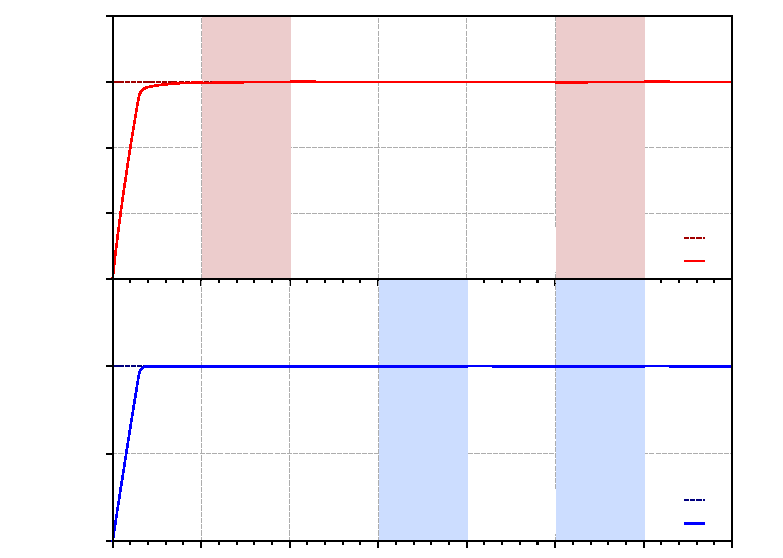
\includegraphics{fado}}%
    \gplfronttext
  \end{picture}%
\endgroup
}
        \vspace{0.5cm}
        \caption{UOAF}
        \label{fig:fado}
    \end{minipage}
\end{figure}

\begin{figure}[htb]
    \begin{minipage}[b]{0.48\linewidth}
        \scalebox{0.65}{% GNUPLOT: LaTeX picture with Postscript
\begingroup
  \makeatletter
  \providecommand\color[2][]{%
    \GenericError{(gnuplot) \space\space\space\@spaces}{%
      Package color not loaded in conjunction with
      terminal option `colourtext'%
    }{See the gnuplot documentation for explanation.%
    }{Either use 'blacktext' in gnuplot or load the package
      color.sty in LaTeX.}%
    \renewcommand\color[2][]{}%
  }%
  \providecommand\includegraphics[2][]{%
    \GenericError{(gnuplot) \space\space\space\@spaces}{%
      Package graphicx or graphics not loaded%
    }{See the gnuplot documentation for explanation.%
    }{The gnuplot epslatex terminal needs graphicx.sty or graphics.sty.}%
    \renewcommand\includegraphics[2][]{}%
  }%
  \providecommand\rotatebox[2]{#2}%
  \@ifundefined{ifGPcolor}{%
    \newif\ifGPcolor
    \GPcolortrue
  }{}%
  \@ifundefined{ifGPblacktext}{%
    \newif\ifGPblacktext
    \GPblacktexttrue
  }{}%
  % define a \g@addto@macro without @ in the name:
  \let\gplgaddtomacro\g@addto@macro
  % define empty templates for all commands taking text:
  \gdef\gplbacktext{}%
  \gdef\gplfronttext{}%
  \makeatother
  \ifGPblacktext
    % no textcolor at all
    \def\colorrgb#1{}%
    \def\colorgray#1{}%
  \else
    % gray or color?
    \ifGPcolor
      \def\colorrgb#1{\color[rgb]{#1}}%
      \def\colorgray#1{\color[gray]{#1}}%
      \expandafter\def\csname LTw\endcsname{\color{white}}%
      \expandafter\def\csname LTb\endcsname{\color{black}}%
      \expandafter\def\csname LTa\endcsname{\color{black}}%
      \expandafter\def\csname LT0\endcsname{\color[rgb]{1,0,0}}%
      \expandafter\def\csname LT1\endcsname{\color[rgb]{0,1,0}}%
      \expandafter\def\csname LT2\endcsname{\color[rgb]{0,0,1}}%
      \expandafter\def\csname LT3\endcsname{\color[rgb]{1,0,1}}%
      \expandafter\def\csname LT4\endcsname{\color[rgb]{0,1,1}}%
      \expandafter\def\csname LT5\endcsname{\color[rgb]{1,1,0}}%
      \expandafter\def\csname LT6\endcsname{\color[rgb]{0,0,0}}%
      \expandafter\def\csname LT7\endcsname{\color[rgb]{1,0.3,0}}%
      \expandafter\def\csname LT8\endcsname{\color[rgb]{0.5,0.5,0.5}}%
    \else
      % gray
      \def\colorrgb#1{\color{black}}%
      \def\colorgray#1{\color[gray]{#1}}%
      \expandafter\def\csname LTw\endcsname{\color{white}}%
      \expandafter\def\csname LTb\endcsname{\color{black}}%
      \expandafter\def\csname LTa\endcsname{\color{black}}%
      \expandafter\def\csname LT0\endcsname{\color{black}}%
      \expandafter\def\csname LT1\endcsname{\color{black}}%
      \expandafter\def\csname LT2\endcsname{\color{black}}%
      \expandafter\def\csname LT3\endcsname{\color{black}}%
      \expandafter\def\csname LT4\endcsname{\color{black}}%
      \expandafter\def\csname LT5\endcsname{\color{black}}%
      \expandafter\def\csname LT6\endcsname{\color{black}}%
      \expandafter\def\csname LT7\endcsname{\color{black}}%
      \expandafter\def\csname LT8\endcsname{\color{black}}%
    \fi
  \fi
  \setlength{\unitlength}{0.0500bp}%
  \begin{picture}(7200.00,5040.00)%
    \gplgaddtomacro\gplbacktext{%
      \csname LTb\endcsname%
      \put(726,3150){\makebox(0,0)[r]{\strut{} 5}}%
      \csname LTb\endcsname%
      \put(726,3780){\makebox(0,0)[r]{\strut{} 10}}%
      \csname LTb\endcsname%
      \put(726,4409){\makebox(0,0)[r]{\strut{} 15}}%
      \csname LTb\endcsname%
      \put(726,5039){\makebox(0,0)[r]{\strut{} 20}}%
      \csname LTb\endcsname%
      \put(921,2237){\makebox(0,0){\strut{}}}%
      \csname LTb\endcsname%
      \put(1771,2237){\makebox(0,0){\strut{}}}%
      \csname LTb\endcsname%
      \put(2620,2237){\makebox(0,0){\strut{}}}%
      \csname LTb\endcsname%
      \put(3470,2237){\makebox(0,0){\strut{}}}%
      \csname LTb\endcsname%
      \put(4320,2237){\makebox(0,0){\strut{}}}%
      \csname LTb\endcsname%
      \put(5170,2237){\makebox(0,0){\strut{}}}%
      \csname LTb\endcsname%
      \put(6019,2237){\makebox(0,0){\strut{}}}%
      \csname LTb\endcsname%
      \put(6869,2237){\makebox(0,0){\strut{}}}%
      \put(352,3779){\rotatebox{-270}{\makebox(0,0){\strut{}Nível [cm]}}}%
    }%
    \gplgaddtomacro\gplfronttext{%
      \csname LTb\endcsname%
      \put(6278,2913){\makebox(0,0)[r]{\strut{}Ref. $T_1$}}%
      \csname LTb\endcsname%
      \put(6278,2693){\makebox(0,0)[r]{\strut{}Saída $T_1$}}%
    }%
    \gplgaddtomacro\gplbacktext{%
      \csname LTb\endcsname%
      \put(726,0){\makebox(0,0)[r]{\strut{} 0}}%
      \csname LTb\endcsname%
      \put(726,840){\makebox(0,0)[r]{\strut{} 10}}%
      \csname LTb\endcsname%
      \put(726,1680){\makebox(0,0)[r]{\strut{} 20}}%
      \csname LTb\endcsname%
      \put(726,2520){\makebox(0,0)[r]{\strut{} 30}}%
      \csname LTb\endcsname%
      \put(921,-283){\makebox(0,0){\strut{}0}}%
      \csname LTb\endcsname%
      \put(1771,-283){\makebox(0,0){\strut{}15}}%
      \csname LTb\endcsname%
      \put(2620,-283){\makebox(0,0){\strut{}30}}%
      \csname LTb\endcsname%
      \put(3470,-283){\makebox(0,0){\strut{}45}}%
      \csname LTb\endcsname%
      \put(4320,-283){\makebox(0,0){\strut{}60}}%
      \csname LTb\endcsname%
      \put(5170,-283){\makebox(0,0){\strut{}75}}%
      \csname LTb\endcsname%
      \put(6019,-283){\makebox(0,0){\strut{}90}}%
      \csname LTb\endcsname%
      \put(6869,-283){\makebox(0,0){\strut{}105}}%
      \put(352,1260){\rotatebox{-270}{\makebox(0,0){\strut{}Nível [cm]}}}%
      \put(3895,-613){\makebox(0,0){\strut{}Tempo [s]}}%
    }%
    \gplgaddtomacro\gplfronttext{%
      \csname LTb\endcsname%
      \put(6278,393){\makebox(0,0)[r]{\strut{}Ref. $T_2$}}%
      \csname LTb\endcsname%
      \put(6278,173){\makebox(0,0)[r]{\strut{}Saída $T_2$}}%
    }%
    \gplbacktext
    \put(0,0){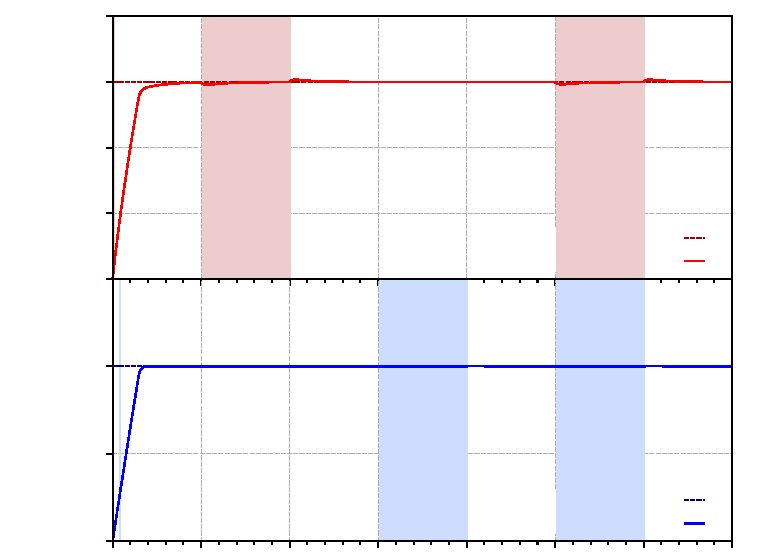
\includegraphics{favk}}%
    \gplfronttext
  \end{picture}%
\endgroup
}
        \vspace{0.5cm}
        \caption{$K_m$AF}
        \label{fig:favk}
    \end{minipage}
    \hfill
    \begin{minipage}[b]{0.48\linewidth}
        \scalebox{0.65}{% GNUPLOT: LaTeX picture with Postscript
\begingroup
  \makeatletter
  \providecommand\color[2][]{%
    \GenericError{(gnuplot) \space\space\space\@spaces}{%
      Package color not loaded in conjunction with
      terminal option `colourtext'%
    }{See the gnuplot documentation for explanation.%
    }{Either use 'blacktext' in gnuplot or load the package
      color.sty in LaTeX.}%
    \renewcommand\color[2][]{}%
  }%
  \providecommand\includegraphics[2][]{%
    \GenericError{(gnuplot) \space\space\space\@spaces}{%
      Package graphicx or graphics not loaded%
    }{See the gnuplot documentation for explanation.%
    }{The gnuplot epslatex terminal needs graphicx.sty or graphics.sty.}%
    \renewcommand\includegraphics[2][]{}%
  }%
  \providecommand\rotatebox[2]{#2}%
  \@ifundefined{ifGPcolor}{%
    \newif\ifGPcolor
    \GPcolortrue
  }{}%
  \@ifundefined{ifGPblacktext}{%
    \newif\ifGPblacktext
    \GPblacktexttrue
  }{}%
  % define a \g@addto@macro without @ in the name:
  \let\gplgaddtomacro\g@addto@macro
  % define empty templates for all commands taking text:
  \gdef\gplbacktext{}%
  \gdef\gplfronttext{}%
  \makeatother
  \ifGPblacktext
    % no textcolor at all
    \def\colorrgb#1{}%
    \def\colorgray#1{}%
  \else
    % gray or color?
    \ifGPcolor
      \def\colorrgb#1{\color[rgb]{#1}}%
      \def\colorgray#1{\color[gray]{#1}}%
      \expandafter\def\csname LTw\endcsname{\color{white}}%
      \expandafter\def\csname LTb\endcsname{\color{black}}%
      \expandafter\def\csname LTa\endcsname{\color{black}}%
      \expandafter\def\csname LT0\endcsname{\color[rgb]{1,0,0}}%
      \expandafter\def\csname LT1\endcsname{\color[rgb]{0,1,0}}%
      \expandafter\def\csname LT2\endcsname{\color[rgb]{0,0,1}}%
      \expandafter\def\csname LT3\endcsname{\color[rgb]{1,0,1}}%
      \expandafter\def\csname LT4\endcsname{\color[rgb]{0,1,1}}%
      \expandafter\def\csname LT5\endcsname{\color[rgb]{1,1,0}}%
      \expandafter\def\csname LT6\endcsname{\color[rgb]{0,0,0}}%
      \expandafter\def\csname LT7\endcsname{\color[rgb]{1,0.3,0}}%
      \expandafter\def\csname LT8\endcsname{\color[rgb]{0.5,0.5,0.5}}%
    \else
      % gray
      \def\colorrgb#1{\color{black}}%
      \def\colorgray#1{\color[gray]{#1}}%
      \expandafter\def\csname LTw\endcsname{\color{white}}%
      \expandafter\def\csname LTb\endcsname{\color{black}}%
      \expandafter\def\csname LTa\endcsname{\color{black}}%
      \expandafter\def\csname LT0\endcsname{\color{black}}%
      \expandafter\def\csname LT1\endcsname{\color{black}}%
      \expandafter\def\csname LT2\endcsname{\color{black}}%
      \expandafter\def\csname LT3\endcsname{\color{black}}%
      \expandafter\def\csname LT4\endcsname{\color{black}}%
      \expandafter\def\csname LT5\endcsname{\color{black}}%
      \expandafter\def\csname LT6\endcsname{\color{black}}%
      \expandafter\def\csname LT7\endcsname{\color{black}}%
      \expandafter\def\csname LT8\endcsname{\color{black}}%
    \fi
  \fi
  \setlength{\unitlength}{0.0500bp}%
  \begin{picture}(7200.00,5040.00)%
    \gplgaddtomacro\gplbacktext{%
      \csname LTb\endcsname%
      \put(726,3150){\makebox(0,0)[r]{\strut{} 5}}%
      \csname LTb\endcsname%
      \put(726,3780){\makebox(0,0)[r]{\strut{} 10}}%
      \csname LTb\endcsname%
      \put(726,4409){\makebox(0,0)[r]{\strut{} 15}}%
      \csname LTb\endcsname%
      \put(726,5039){\makebox(0,0)[r]{\strut{} 20}}%
      \csname LTb\endcsname%
      \put(921,2237){\makebox(0,0){\strut{}}}%
      \csname LTb\endcsname%
      \put(1771,2237){\makebox(0,0){\strut{}}}%
      \csname LTb\endcsname%
      \put(2620,2237){\makebox(0,0){\strut{}}}%
      \csname LTb\endcsname%
      \put(3470,2237){\makebox(0,0){\strut{}}}%
      \csname LTb\endcsname%
      \put(4320,2237){\makebox(0,0){\strut{}}}%
      \csname LTb\endcsname%
      \put(5170,2237){\makebox(0,0){\strut{}}}%
      \csname LTb\endcsname%
      \put(6019,2237){\makebox(0,0){\strut{}}}%
      \csname LTb\endcsname%
      \put(6869,2237){\makebox(0,0){\strut{}}}%
      \put(352,3779){\rotatebox{-270}{\makebox(0,0){\strut{}Level [cm]}}}%
    }%
    \gplgaddtomacro\gplfronttext{%
      \csname LTb\endcsname%
      \put(6278,2913){\makebox(0,0)[r]{\strut{}Setpoint $T_1$}}%
      \csname LTb\endcsname%
      \put(6278,2693){\makebox(0,0)[r]{\strut{}Output $T_1$}}%
    }%
    \gplgaddtomacro\gplbacktext{%
      \csname LTb\endcsname%
      \put(726,0){\makebox(0,0)[r]{\strut{} 0}}%
      \csname LTb\endcsname%
      \put(726,840){\makebox(0,0)[r]{\strut{} 10}}%
      \csname LTb\endcsname%
      \put(726,1680){\makebox(0,0)[r]{\strut{} 20}}%
      \csname LTb\endcsname%
      \put(726,2520){\makebox(0,0)[r]{\strut{} 30}}%
      \csname LTb\endcsname%
      \put(921,-283){\makebox(0,0){\strut{}0}}%
      \csname LTb\endcsname%
      \put(1771,-283){\makebox(0,0){\strut{}15}}%
      \csname LTb\endcsname%
      \put(2620,-283){\makebox(0,0){\strut{}30}}%
      \csname LTb\endcsname%
      \put(3470,-283){\makebox(0,0){\strut{}45}}%
      \csname LTb\endcsname%
      \put(4320,-283){\makebox(0,0){\strut{}60}}%
      \csname LTb\endcsname%
      \put(5170,-283){\makebox(0,0){\strut{}75}}%
      \csname LTb\endcsname%
      \put(6019,-283){\makebox(0,0){\strut{}90}}%
      \csname LTb\endcsname%
      \put(6869,-283){\makebox(0,0){\strut{}105}}%
      \put(352,1260){\rotatebox{-270}{\makebox(0,0){\strut{}Level [cm]}}}%
      \put(3895,-613){\makebox(0,0){\strut{}Time [s]}}%
    }%
    \gplgaddtomacro\gplfronttext{%
      \csname LTb\endcsname%
      \put(6278,393){\makebox(0,0)[r]{\strut{}Setpoint $T_2$}}%
      \csname LTb\endcsname%
      \put(6278,173){\makebox(0,0)[r]{\strut{}Output $T_2$}}%
    }%
    \gplbacktext
    \put(0,0){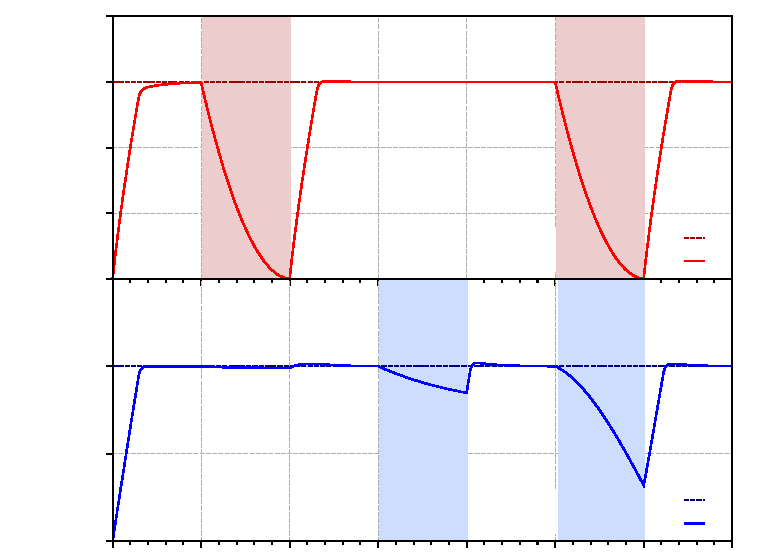
\includegraphics{faq}}%
    \gplfronttext
  \end{picture}%
\endgroup
}
        \vspace{0.5cm}
        \caption{BAF}
        \label{fig:faq}
    \end{minipage}
\end{figure}

\begin{figure}[htb]
    \begin{minipage}[b]{0.48\linewidth}
        \scalebox{0.65}{% GNUPLOT: LaTeX picture with Postscript
\begingroup
  \makeatletter
  \providecommand\color[2][]{%
    \GenericError{(gnuplot) \space\space\space\@spaces}{%
      Package color not loaded in conjunction with
      terminal option `colourtext'%
    }{See the gnuplot documentation for explanation.%
    }{Either use 'blacktext' in gnuplot or load the package
      color.sty in LaTeX.}%
    \renewcommand\color[2][]{}%
  }%
  \providecommand\includegraphics[2][]{%
    \GenericError{(gnuplot) \space\space\space\@spaces}{%
      Package graphicx or graphics not loaded%
    }{See the gnuplot documentation for explanation.%
    }{The gnuplot epslatex terminal needs graphicx.sty or graphics.sty.}%
    \renewcommand\includegraphics[2][]{}%
  }%
  \providecommand\rotatebox[2]{#2}%
  \@ifundefined{ifGPcolor}{%
    \newif\ifGPcolor
    \GPcolortrue
  }{}%
  \@ifundefined{ifGPblacktext}{%
    \newif\ifGPblacktext
    \GPblacktexttrue
  }{}%
  % define a \g@addto@macro without @ in the name:
  \let\gplgaddtomacro\g@addto@macro
  % define empty templates for all commands taking text:
  \gdef\gplbacktext{}%
  \gdef\gplfronttext{}%
  \makeatother
  \ifGPblacktext
    % no textcolor at all
    \def\colorrgb#1{}%
    \def\colorgray#1{}%
  \else
    % gray or color?
    \ifGPcolor
      \def\colorrgb#1{\color[rgb]{#1}}%
      \def\colorgray#1{\color[gray]{#1}}%
      \expandafter\def\csname LTw\endcsname{\color{white}}%
      \expandafter\def\csname LTb\endcsname{\color{black}}%
      \expandafter\def\csname LTa\endcsname{\color{black}}%
      \expandafter\def\csname LT0\endcsname{\color[rgb]{1,0,0}}%
      \expandafter\def\csname LT1\endcsname{\color[rgb]{0,1,0}}%
      \expandafter\def\csname LT2\endcsname{\color[rgb]{0,0,1}}%
      \expandafter\def\csname LT3\endcsname{\color[rgb]{1,0,1}}%
      \expandafter\def\csname LT4\endcsname{\color[rgb]{0,1,1}}%
      \expandafter\def\csname LT5\endcsname{\color[rgb]{1,1,0}}%
      \expandafter\def\csname LT6\endcsname{\color[rgb]{0,0,0}}%
      \expandafter\def\csname LT7\endcsname{\color[rgb]{1,0.3,0}}%
      \expandafter\def\csname LT8\endcsname{\color[rgb]{0.5,0.5,0.5}}%
    \else
      % gray
      \def\colorrgb#1{\color{black}}%
      \def\colorgray#1{\color[gray]{#1}}%
      \expandafter\def\csname LTw\endcsname{\color{white}}%
      \expandafter\def\csname LTb\endcsname{\color{black}}%
      \expandafter\def\csname LTa\endcsname{\color{black}}%
      \expandafter\def\csname LT0\endcsname{\color{black}}%
      \expandafter\def\csname LT1\endcsname{\color{black}}%
      \expandafter\def\csname LT2\endcsname{\color{black}}%
      \expandafter\def\csname LT3\endcsname{\color{black}}%
      \expandafter\def\csname LT4\endcsname{\color{black}}%
      \expandafter\def\csname LT5\endcsname{\color{black}}%
      \expandafter\def\csname LT6\endcsname{\color{black}}%
      \expandafter\def\csname LT7\endcsname{\color{black}}%
      \expandafter\def\csname LT8\endcsname{\color{black}}%
    \fi
  \fi
  \setlength{\unitlength}{0.0500bp}%
  \begin{picture}(7200.00,5040.00)%
    \gplgaddtomacro\gplbacktext{%
      \csname LTb\endcsname%
      \put(726,3150){\makebox(0,0)[r]{\strut{} 5}}%
      \csname LTb\endcsname%
      \put(726,3780){\makebox(0,0)[r]{\strut{} 10}}%
      \csname LTb\endcsname%
      \put(726,4409){\makebox(0,0)[r]{\strut{} 15}}%
      \csname LTb\endcsname%
      \put(726,5039){\makebox(0,0)[r]{\strut{} 20}}%
      \csname LTb\endcsname%
      \put(921,2237){\makebox(0,0){\strut{}}}%
      \csname LTb\endcsname%
      \put(1771,2237){\makebox(0,0){\strut{}}}%
      \csname LTb\endcsname%
      \put(2620,2237){\makebox(0,0){\strut{}}}%
      \csname LTb\endcsname%
      \put(3470,2237){\makebox(0,0){\strut{}}}%
      \csname LTb\endcsname%
      \put(4320,2237){\makebox(0,0){\strut{}}}%
      \csname LTb\endcsname%
      \put(5170,2237){\makebox(0,0){\strut{}}}%
      \csname LTb\endcsname%
      \put(6019,2237){\makebox(0,0){\strut{}}}%
      \csname LTb\endcsname%
      \put(6869,2237){\makebox(0,0){\strut{}}}%
      \put(352,3779){\rotatebox{-270}{\makebox(0,0){\strut{}Level [cm]}}}%
    }%
    \gplgaddtomacro\gplfronttext{%
      \csname LTb\endcsname%
      \put(6278,2913){\makebox(0,0)[r]{\strut{}Setpoint $T_1$}}%
      \csname LTb\endcsname%
      \put(6278,2693){\makebox(0,0)[r]{\strut{}Output $T_1$}}%
    }%
    \gplgaddtomacro\gplbacktext{%
      \csname LTb\endcsname%
      \put(726,0){\makebox(0,0)[r]{\strut{} 0}}%
      \csname LTb\endcsname%
      \put(726,840){\makebox(0,0)[r]{\strut{} 10}}%
      \csname LTb\endcsname%
      \put(726,1680){\makebox(0,0)[r]{\strut{} 20}}%
      \csname LTb\endcsname%
      \put(726,2520){\makebox(0,0)[r]{\strut{} 30}}%
      \csname LTb\endcsname%
      \put(921,-283){\makebox(0,0){\strut{}0}}%
      \csname LTb\endcsname%
      \put(1771,-283){\makebox(0,0){\strut{}15}}%
      \csname LTb\endcsname%
      \put(2620,-283){\makebox(0,0){\strut{}30}}%
      \csname LTb\endcsname%
      \put(3470,-283){\makebox(0,0){\strut{}45}}%
      \csname LTb\endcsname%
      \put(4320,-283){\makebox(0,0){\strut{}60}}%
      \csname LTb\endcsname%
      \put(5170,-283){\makebox(0,0){\strut{}75}}%
      \csname LTb\endcsname%
      \put(6019,-283){\makebox(0,0){\strut{}90}}%
      \csname LTb\endcsname%
      \put(6869,-283){\makebox(0,0){\strut{}105}}%
      \put(352,1260){\rotatebox{-270}{\makebox(0,0){\strut{}Level [cm]}}}%
      \put(3895,-613){\makebox(0,0){\strut{}Time [s]}}%
    }%
    \gplgaddtomacro\gplfronttext{%
      \csname LTb\endcsname%
      \put(6278,393){\makebox(0,0)[r]{\strut{}Setpoint $T_2$}}%
      \csname LTb\endcsname%
      \put(6278,173){\makebox(0,0)[r]{\strut{}Output $T_2$}}%
    }%
    \gplbacktext
    \put(0,0){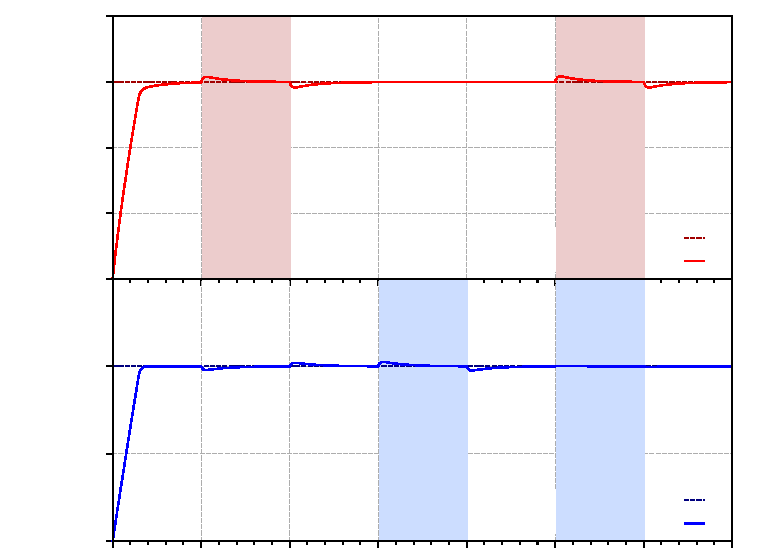
\includegraphics{fsieos}}%
    \gplfronttext
  \end{picture}%
\endgroup
}
        \vspace{0.5cm}
        \caption{T$a_i$OStF}
        \label{fig:fsieos}
    \end{minipage}
    \hfill
    \begin{minipage}[b]{0.48\linewidth}
        \scalebox{0.65}{% GNUPLOT: LaTeX picture with Postscript
\begingroup
  \makeatletter
  \providecommand\color[2][]{%
    \GenericError{(gnuplot) \space\space\space\@spaces}{%
      Package color not loaded in conjunction with
      terminal option `colourtext'%
    }{See the gnuplot documentation for explanation.%
    }{Either use 'blacktext' in gnuplot or load the package
      color.sty in LaTeX.}%
    \renewcommand\color[2][]{}%
  }%
  \providecommand\includegraphics[2][]{%
    \GenericError{(gnuplot) \space\space\space\@spaces}{%
      Package graphicx or graphics not loaded%
    }{See the gnuplot documentation for explanation.%
    }{The gnuplot epslatex terminal needs graphicx.sty or graphics.sty.}%
    \renewcommand\includegraphics[2][]{}%
  }%
  \providecommand\rotatebox[2]{#2}%
  \@ifundefined{ifGPcolor}{%
    \newif\ifGPcolor
    \GPcolortrue
  }{}%
  \@ifundefined{ifGPblacktext}{%
    \newif\ifGPblacktext
    \GPblacktexttrue
  }{}%
  % define a \g@addto@macro without @ in the name:
  \let\gplgaddtomacro\g@addto@macro
  % define empty templates for all commands taking text:
  \gdef\gplbacktext{}%
  \gdef\gplfronttext{}%
  \makeatother
  \ifGPblacktext
    % no textcolor at all
    \def\colorrgb#1{}%
    \def\colorgray#1{}%
  \else
    % gray or color?
    \ifGPcolor
      \def\colorrgb#1{\color[rgb]{#1}}%
      \def\colorgray#1{\color[gray]{#1}}%
      \expandafter\def\csname LTw\endcsname{\color{white}}%
      \expandafter\def\csname LTb\endcsname{\color{black}}%
      \expandafter\def\csname LTa\endcsname{\color{black}}%
      \expandafter\def\csname LT0\endcsname{\color[rgb]{1,0,0}}%
      \expandafter\def\csname LT1\endcsname{\color[rgb]{0,1,0}}%
      \expandafter\def\csname LT2\endcsname{\color[rgb]{0,0,1}}%
      \expandafter\def\csname LT3\endcsname{\color[rgb]{1,0,1}}%
      \expandafter\def\csname LT4\endcsname{\color[rgb]{0,1,1}}%
      \expandafter\def\csname LT5\endcsname{\color[rgb]{1,1,0}}%
      \expandafter\def\csname LT6\endcsname{\color[rgb]{0,0,0}}%
      \expandafter\def\csname LT7\endcsname{\color[rgb]{1,0.3,0}}%
      \expandafter\def\csname LT8\endcsname{\color[rgb]{0.5,0.5,0.5}}%
    \else
      % gray
      \def\colorrgb#1{\color{black}}%
      \def\colorgray#1{\color[gray]{#1}}%
      \expandafter\def\csname LTw\endcsname{\color{white}}%
      \expandafter\def\csname LTb\endcsname{\color{black}}%
      \expandafter\def\csname LTa\endcsname{\color{black}}%
      \expandafter\def\csname LT0\endcsname{\color{black}}%
      \expandafter\def\csname LT1\endcsname{\color{black}}%
      \expandafter\def\csname LT2\endcsname{\color{black}}%
      \expandafter\def\csname LT3\endcsname{\color{black}}%
      \expandafter\def\csname LT4\endcsname{\color{black}}%
      \expandafter\def\csname LT5\endcsname{\color{black}}%
      \expandafter\def\csname LT6\endcsname{\color{black}}%
      \expandafter\def\csname LT7\endcsname{\color{black}}%
      \expandafter\def\csname LT8\endcsname{\color{black}}%
    \fi
  \fi
  \setlength{\unitlength}{0.0500bp}%
  \begin{picture}(7200.00,5040.00)%
    \gplgaddtomacro\gplbacktext{%
      \csname LTb\endcsname%
      \put(726,3150){\makebox(0,0)[r]{\strut{} 5}}%
      \csname LTb\endcsname%
      \put(726,3780){\makebox(0,0)[r]{\strut{} 10}}%
      \csname LTb\endcsname%
      \put(726,4409){\makebox(0,0)[r]{\strut{} 15}}%
      \csname LTb\endcsname%
      \put(726,5039){\makebox(0,0)[r]{\strut{} 20}}%
      \csname LTb\endcsname%
      \put(921,2237){\makebox(0,0){\strut{}}}%
      \csname LTb\endcsname%
      \put(1771,2237){\makebox(0,0){\strut{}}}%
      \csname LTb\endcsname%
      \put(2620,2237){\makebox(0,0){\strut{}}}%
      \csname LTb\endcsname%
      \put(3470,2237){\makebox(0,0){\strut{}}}%
      \csname LTb\endcsname%
      \put(4320,2237){\makebox(0,0){\strut{}}}%
      \csname LTb\endcsname%
      \put(5170,2237){\makebox(0,0){\strut{}}}%
      \csname LTb\endcsname%
      \put(6019,2237){\makebox(0,0){\strut{}}}%
      \csname LTb\endcsname%
      \put(6869,2237){\makebox(0,0){\strut{}}}%
      \put(352,3779){\rotatebox{-270}{\makebox(0,0){\strut{}Nível [cm]}}}%
    }%
    \gplgaddtomacro\gplfronttext{%
      \csname LTb\endcsname%
      \put(6278,2913){\makebox(0,0)[r]{\strut{}Ref. $T_1$}}%
      \csname LTb\endcsname%
      \put(6278,2693){\makebox(0,0)[r]{\strut{}Saída $T_1$}}%
    }%
    \gplgaddtomacro\gplbacktext{%
      \csname LTb\endcsname%
      \put(726,0){\makebox(0,0)[r]{\strut{} 0}}%
      \csname LTb\endcsname%
      \put(726,840){\makebox(0,0)[r]{\strut{} 10}}%
      \csname LTb\endcsname%
      \put(726,1680){\makebox(0,0)[r]{\strut{} 20}}%
      \csname LTb\endcsname%
      \put(726,2520){\makebox(0,0)[r]{\strut{} 30}}%
      \csname LTb\endcsname%
      \put(921,-283){\makebox(0,0){\strut{}0}}%
      \csname LTb\endcsname%
      \put(1771,-283){\makebox(0,0){\strut{}15}}%
      \csname LTb\endcsname%
      \put(2620,-283){\makebox(0,0){\strut{}30}}%
      \csname LTb\endcsname%
      \put(3470,-283){\makebox(0,0){\strut{}45}}%
      \csname LTb\endcsname%
      \put(4320,-283){\makebox(0,0){\strut{}60}}%
      \csname LTb\endcsname%
      \put(5170,-283){\makebox(0,0){\strut{}75}}%
      \csname LTb\endcsname%
      \put(6019,-283){\makebox(0,0){\strut{}90}}%
      \csname LTb\endcsname%
      \put(6869,-283){\makebox(0,0){\strut{}105}}%
      \put(352,1260){\rotatebox{-270}{\makebox(0,0){\strut{}Nível [cm]}}}%
      \put(3895,-613){\makebox(0,0){\strut{}Tempo [s]}}%
    }%
    \gplgaddtomacro\gplfronttext{%
      \csname LTb\endcsname%
      \put(6278,393){\makebox(0,0)[r]{\strut{}Ref. $T_2$}}%
      \csname LTb\endcsname%
      \put(6278,173){\makebox(0,0)[r]{\strut{}Saída $T_2$}}%
    }%
    \gplbacktext
    \put(0,0){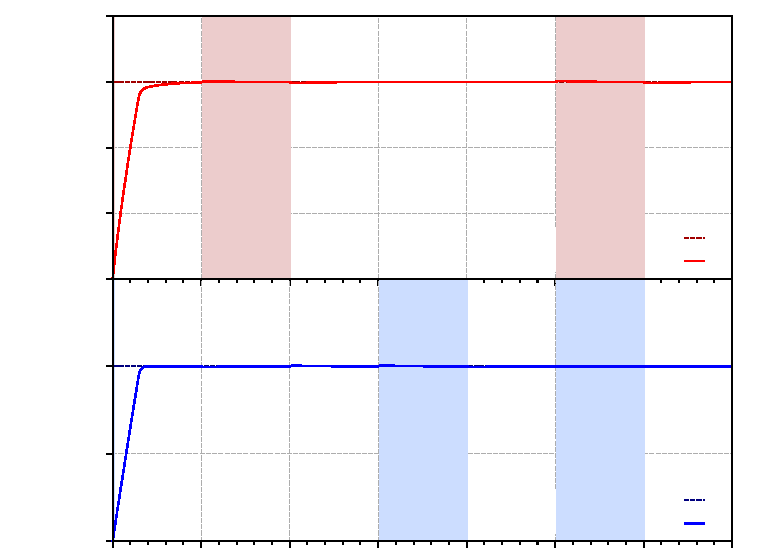
\includegraphics{fsivros}}%
    \gplfronttext
  \end{picture}%
\endgroup
}
        \vspace{0.5cm}
        \caption{T$a_i$VStF}
        \label{fig:fsivros}
    \end{minipage}
\end{figure}

\begin{comment}
Uma última observação pode ser feita a respeito da Fig. \ref{fig:fseq}, em que
há a detecção da falha em $T_1$ em um pequeno intervalo no final da simulação.
Contudo, isso não veio a comprometer o funcionamento do sistema nos intervalos
em que a falha deveria realmente ser detectada. Trata-se, portanto, de um falso
positivo.
\end{comment}

Ressalta-se por fim que as situações adversas podem ter ocorrido no sistema em
virtude do treinamento ter sido realizado com valores constantes para a variação
dos parâmetros. Por esse motivo os resultados obtidos nem sempre estão de acordo
com os valores da Tab. \ref{tab:best_ann}.

% ==============================================================================
% CONCLUSIONS
% ==============================================================================
\section{CONCLUSIONS}\label{sec:conclusions}
O presente trabalho foi desenvolvido com o intuito de fornecer um sistema DDF
para um sistema de tanques acoplados. Para isso, o sistema fez uso de uma
estrutura neural que, a partir dos valores disponíveis, indicava ao usuário os
momentos em que as falhas estavam ocorrendo. 

Tal estrutura, por ser completamente desarticulada, abre margem para que outras
técnicas de detecção e diagnóstico venham a ser utilizadas para falhas
específicas, substituindo aquelas redes que tiverem desempenho aquém ao
esperado.

Dentre as falhas selecionadas, oito foram identificadas com facilidade e outras
três tiveram um desempenho satisfatório, com um pequeno problema de detecção que
pode ser facilmente resolvido através de {\it flags} binárias. As outras duas
falhas não foram identificadas corretamente, mas, em ambos os casos, o sistema
consegue detectar a falha corretamente para $T_1$.

Observa-se ainda que os resultados obtidos podem melhorar ainda mais quando
forem utilizados valores reais, oscilando dentro da faixa de valores em que a
rede foi treinada. Tal situação pode fazer com que não mais ocorra o problema de
detecção das UGSeF, UOSeF e TLStF, evitando portanto a utilização de {\it
flags} para contorná-lo.

Assim, pode-se dizer que o sistema teve um desempenho satisfatório, conseguindo
identificar cerca de 85\% das falhas propostas. Comprova-se, portanto, que as
redes neurais de múltiplas camadas são estruturas eficientes tanto para a
identificação de modelos quanto para a detecção e o diagnóstico de falhas.

Uma vez que o sistema tenha sido testado com vários sinais de excitação, pode-se
então acoplá-lo à um sistema de controle tolerante à falhas (SCTF). Nesse caso
os sinais gerados pelo sistema de DDF servirão como ``alarmes''. O SCTF, por sua
vez, poderá realizar a reconfiguração dos controladores, modificando os valores
dos ganhos ou até mesmo suas estruturas, de tal forma que o sistema continue
funcionando de maneira correta até que a falha tenha sido corrigida.

% ==============================================================================
% ACKNOWLEDGEMENTS
% ==============================================================================
\begin{comment}
\section{ACKNOWLEDGEMENTS}
The authors thank CAPES for financial support and also the colleagues in ITA and
UFPA.
\end{comment}

% ==============================================================================
% REFERENCES
% ==============================================================================
\section{REFERENCES}

\bibliographystyle{cobem}
\renewcommand{\refname}{}
\bibliography{bibfile}

\end{document}
